\documentclass[pdflatex,sn-basic]{sn-jnl}

\usepackage{graphicx}%
\usepackage[export]{adjustbox}%
\usepackage{multirow}%
\usepackage{amsmath,amssymb,amsfonts}%
\usepackage{amsthm}%
\usepackage{mathrsfs}%
\usepackage[title]{appendix}%
\usepackage{xcolor}%
\usepackage{textcomp}%
\usepackage{manyfoot}%
\usepackage{booktabs}%

\theoremstyle{thmstyleone}%
\newtheorem{proposition}{Proposition}%
\newtheorem{lemma}{Lemma}%

\raggedbottom

\begin{document}

\title[Screening for coordinated manipulation and evaluating exchange rules]{Screening for Coordinated Manipulation and Evaluating Exchange Rules in a Vietnam-Calibrated Market Simulator}

\author*[1]{\fnm{Quang-Vinh} \sur{Dang}}\email{vinh.dq4@buv.edu.vn}
\equalcont{ORCID: 0000-0002-3877-8024}

\affil*[1]{\orgname{British University Vietnam}, \orgaddress{\city{Hung Yen}, \country{Vietnam}}}

\abstract{Prosecuted manipulation on Vietnamese stock exchanges is mostly carried out by groups of accounts trading in step, yet regulators have no labelled cases to train a detector and the order-level data to test one are not public. We study which rules and how much inspection capacity make such a ring give up. We state a label-free coincidence test with an exact circular-shift null per account, derive a power law in which the shift of the statistic falls like the inverse square root of the number of accounts; the law fits an agent-based market and yields a deterrence condition linking inspection capacity to the fine. A ring that re-optimises against each rule across simulated markets matching moments of the Ho Chi Minh Stock Exchange is unaffected by the daily price band, loses most of the block value when off-book blocks are priced at a trailing mean, and is deterred by inspection only with enough capacity; minimum resting times and cancel fees do not deter and raise volatility. On real order flow from a public derivatives venue the exchangeability condition fails for a quarter of the active accounts, and a planted ring of 12 quiet accounts is found only when it makes up about a fifth of the flow. On Vietnamese public data, the 2016 tick reform lowered the share of zero-return days by seven points, and a price-based rank places 8 of 10 documented cases in the daily top ten of 1,360 stocks.}

\keywords{market manipulation, market surveillance, agent-based model, limit order book, exchange rules, Vietnam}

\pacs[JEL Classification]{G18, G14, C63, D47, K42}

\maketitle

\section{Introduction}\label{sec:intro}

A securities regulator that wants to find manipulation faces three problems at once. It rarely has labelled cases, because enforcement is slow and selective. It cannot easily evaluate a rule change before introducing it, because the behaviour of manipulators changes with the rule. And the data that would let an outside researcher test a method, orders tagged with an account, is held only by the exchange and the regulator. These problems are acute in Vietnam. In ten recent decisions of the State Securities Commission with exact dates (Appendix~\ref{app:cases}) the manipulation was carried out with between 5 and 164 accounts (median 24.5), by trading continuously, or crossing orders among accounts, to create the appearance of supply and demand. Spoofing and layering, the focus of most of the detection literature \citep{tuccella2021,fabre2025}, do not appear among these cases.

This paper asks two questions of a regulator in that position and answers them with a combination of theory, simulation and public data. \emph{Can a ring of accounts be found without labelled cases?} And \emph{which rules and how much inspection capacity make a ring that adapts to them give up?} For the first we study a label-free coincidence test: each account's submissions are compared with the aggregate of all other accounts, and the comparison is calibrated by circularly shifting the account's own series, which gives an exact $p$-value under a stated exchangeability condition. For the second we let a ring re-optimise against each rule in a family of simulated markets that match published and measured moments of the Ho Chi Minh Stock Exchange, and we relate the answer to closed-form conditions.

We make six contributions. (i)~We state the test, prove that it controls false alarms exactly per account (Proposition~\ref{prop:exact}), and show that ranking many accounts at once cannot inherit that guarantee because of the resolution of the shift distribution (Proposition~\ref{prop:budget}). (ii)~We derive a law for its power, in which the shift of the statistic falls like $N^{-1/2}$ in the number of accounts and rises with the number of co-active members (Proposition~\ref{prop:power}), verify it by Monte Carlo and show that it explains the dependence on the number of accounts in the agent-based market; we show why netting buys against sells protects against honest market-making desks (Proposition~\ref{prop:netting}). (iii)~We turn the law into a deterrence condition for a regulator with a fixed inspection capacity and a fine proportional to the gain (Proposition~\ref{prop:deter}), and derive and test a law for a rule that prices off-book blocks at a trailing mean (Proposition~\ref{prop:block}). (iv)~We evaluate rules by the best response of a ring over two families of six calibrated markets, with the effect of rules on honest participants (Section~\ref{sec:policy}). (v)~We stress-test the statistic on real account-level order flow from a public venue, where it fails the exchangeability condition for a large share of accounts and detects a planted ring less often than in the simulator (Section~\ref{sec:real-accounts}), and we check what public data on Vietnam can say: documented enforcement cases, a natural experiment on the tick size, and pump events (Section~\ref{sec:real}). (vi)~We release the code and all result tables.

The paper does not claim that the detector works on real Vietnamese order data. Its manipulators and features are written by us, a supervised model trained in the simulator does better than the label-free test in every simulated scenario, the real account-level data come from a different kind of market, and the Vietnamese checks are at the level of the stock, not of the account. The contribution is a calibrated screening tool with a measured failure profile, a theory that links its power to deterrence capacity, and an evaluation method for rules that does not assume manipulators stand still. Section~\ref{sec:related} places the paper among the related work, Section~\ref{sec:sim} sets up the market and the regulator's problem, Section~\ref{sec:method} gives the method and its theory, Sections~\ref{sec:detect}--\ref{sec:real} report the experiments, and Section~\ref{sec:discussion} discusses the impact for policy and the limits.


\section{Related work and position of this paper}\label{sec:related}

Four literatures meet in the problem we study: detecting manipulation, finding coordination among traders, testing coincidence between event series, and using simulated markets and enforcement theory to choose rules. For each we say what it provides, what it assumes, and what is left for this paper; Table~\ref{tab:positioning} summarises.

\paragraph{Detection with labelled events or order-book data.} Most detection work targets a manipulation that leaves a public trace or a label. For pump-and-dump schemes organised on messaging channels the announcement itself labels the event: \citet{xu2019} study 412 pumps announced on Telegram (June 2018 to February 2019) and predict which coin will be pumped; \citet{hu2022} model 709 events from 2019 to 2022 with a sequence network over channel histories; \citet{lamorgia2020} propose a real-time detector and \citet{lamorgia2023} reach an F1 score of 94.5\% with detection 25 seconds after a pump starts, on a data set of about 900 events; \citet{dhawan2023} measure average price distortions of 65\% on 355 cases; \citet{kamps2018} define criteria and apply anomaly detection to trade data. For spoofing, \citet{tuccella2021} train a recurrent network on granular order-book data for early detection, and \citet{fabre2025} predict the distribution of mid-price moves from Hawkes-process order-flow variables and find that 31\% of the large orders in a three-day sample of Level-3 data could spoof. Wash trading is detected from structure: loops of matched orders in directed trader graphs on stock data \citep{cao2016}, accounts and trading structures that meet legal definitions on two blockchain exchanges \citep{victor2021}, and statistical regularities of reported volume, which put wash trading above 70\% of reported volume on unregulated exchanges \citep{cong2023}. These methods need labels (announcements, cases) or counterparty-level records, and the spoofing and pump settings are not those of the Vietnamese cases, in which groups of accounts trade among themselves or continuously for months (Appendix~\ref{app:cases}). We use a pump data set only to measure how weak the preparation phase of a pump is in public tick data (Section~\ref{sec:pump}); our detector uses neither labels nor counterparties, only the timing and side of submissions.

\paragraph{Coordination among traders.} Closer to our setting, collusion has been sought in trade networks. \citet{palshikar2008} cluster the trade graph and combine evidence from several algorithms; \citet{sun2012} test the correlation between the degree and strength of traders in networks of eight manipulated and 44 non-manipulated stocks against randomised networks; \citet{jaeger2025} link insiders by the temporal similarity of their reported trades in 2.9 million filings, motivated precisely by the lack of labels. \citet{saavedra2011} show that synchrony is a common trait of honest traders: day traders who trade more in step with others lose less, so synchrony alone does not signal collusion. That finding is the reason for our emphasis on honest groups (market-making desks, order-splitting funds, bot fleets) and for the netting of buys against sells (Proposition~\ref{prop:netting}), and it is borne out on real order flow (Section~\ref{sec:real-accounts}). Relative to this strand we compare one account with the \emph{aggregate} of all others rather than pairs, which pools evidence when a ring fragments its trading over many accounts, and we attach an exact null to the comparison.

\paragraph{Coincidence tests with surrogates.} Testing whether events in two series coincide more than chance without a model for either series is a long-standing problem in neuroscience. \citet{grun2009} show that nonstationary rates and non-Poisson structure generate false positives unless they are part of the null; \citet{louis2010} build surrogates that keep rates and inter-event intervals; \citet{amarasingham2012} review jitter resampling and exact tests for repeated fine-scale patterns; \citet{platkiewicz2017} prove that interval jitter gives an exact test while spike-centred jitter can inflate false positives; \citet{liang2025} give finite-sample false-positive guarantees for time-shift tests that allow dependence within the series. We transfer the circular-shift version to accounts, add netting, take the maximum over tolerances inside one shift distribution, and prove two properties that matter for a regulator: the resolution limit of the discrete $p$-value across many accounts (Proposition~\ref{prop:budget}) and a power law in the number of accounts (Proposition~\ref{prop:power}). The warning of \citet{grun2009} is the main lesson of our real-data test: common drivers make the null false for most active accounts.

\paragraph{Simulated markets for rules and for surveillance.} Open simulators exist \citep{byrd2020}, and their realism is a recognised issue: \citet{vyetrenko2019} compare simulated and real limit order books on stylised facts and find more realistic behaviour when the fundamental comes from historical data, and \citet{platt2018} find that microstructure parameters of agent-based models can be calibrated but behavioural parameters remain problematic. Both point to the design we adopt, a family of markets matching the observable moments instead of a single tuned market (Section~\ref{sec:br}). Agent-based models have been used to study rules: tick size, which worsens quality, especially for small caps, as it grows \citep{zhao2020}; price limits, which cause volatility spillover and delay price discovery when upper limits bind \citep{zhang2016}; and minimum resting times, circuit breakers, cancellation fees and taxes, which trade stability against resilience in a market with high-frequency traders \citep{leal2019}. For manipulation specifically, \citet{wang2020} generate order streams in which a manipulator mimics a market maker, and \citet{wang2018} analyse a cloaking rule against a spoofing exploiter by empirical game-theoretic analysis; \citet{cartea2020} show in a control model that a larger fine makes spoofing less attractive until it disappears. These studies concern single manipulators and generic markets. We study a ring, a specific venue, and the best response of the manipulator to each rule in a family of calibrated markets, add closed-form conditions (deterrence capacity, block-price law), and verify the mechanism ex post.

\paragraph{Enforcement economics and Vietnamese evidence.} Deterrence depends on the probability of detection and the size of the sanction \citep{becker1968,polinsky2000}; inspection games formalise limited inspection capacity \citep{avenhaus2002}, and double-oracle methods compute equilibria of games with an adversary \citep{mcmahan2003,lanctot2017}, a natural next step for the interaction between an adaptive ring and an adaptive regulator. \citet{aggarwal2006} use SEC cases to show that manipulation raises volatility, liquidity and returns during the episode, with prices falling afterwards; \citet{comerton2014} estimate that about 1\% of closing prices are manipulated, that only a small fraction is detected and prosecuted, and that the regulator's budget has a strong effect on both manipulation and detection, which is the empirical counterpart of our capacity result (Proposition~\ref{prop:deter}); \citet{khwaja2005} study price manipulation by intermediaries in an emerging market. For Vietnam, \citet{nguyen2017} study insider trading around stock splits, \citet{nguyen2023} herding across COVID-19 periods, and \citet{vo2023} find that the 2016 tick reduction lowered trading costs on the Ho Chi Minh Stock Exchange, a result we use as an external check (Section~\ref{sec:tick}). None of these studies has account-level manipulation data for Vietnam, and neither do we.

\begin{table}[t]
\centering\footnotesize
\begin{adjustbox}{max width=\linewidth}
\begin{tabular}{p{3.6cm}p{3.4cm}p{1.4cm}p{1.6cm}p{2.3cm}p{1.8cm}}
\toprule
strand & typical input & labels needed & account-level data & error control & policy evaluation\\
\midrule
pump-and-dump detection & public tick data and announcements & yes & no & empirical & no\\
spoofing detection & order book, orders & yes & no (one trader) & empirical & little\\
wash-trading detection & counterparty-level trades & rules or labels & yes & rules, empirical & no\\
trader-network collusion & trade graphs, filings & some & yes & randomised networks & no\\
time-shift and jitter tests & event series (neuroscience) & no & not applicable & exact or finite-sample & no\\
agent-based rule studies & simulated markets & no & simulated & not applicable & yes, fixed agents\\
\textbf{this paper} & order submissions (time, side) & no & yes (not public here) & exact per account; ranking in practice & yes, best response over calibrated markets\\
\bottomrule
\end{tabular}
\end{adjustbox}
\caption{Positioning of the paper among the strands of related work.}\label{tab:positioning}
\end{table}

\paragraph{Position.} The gap this paper addresses is the combination of the strands in the last row: a screening statistic that needs neither labels nor counterparties, whose error properties and power are stated and checked, together with a policy evaluation in which the manipulator adapts and the market is not a single draw. Our claims are limited accordingly. Components are not new (shift tests, adversarial simulation, enforcement economics); the contribution is their calibrated combination, the theory that connects detection power to deterrence capacity and to the effect of a block-price rule, and the measurement of where the combination fails, on simulated honest groups and on real account-level order flow.


\section{Setting: a calibrated market, a ring and a regulator}\label{sec:sim}

\subsection{The market and the manipulators}\label{sec:market}

\paragraph{Market.} A limit order book with price-time priority and self-trade prevention; one step is about one trading minute and a day has 240 steps. Honest agents are noise traders, market makers that re-quote two levels per side and shift with displayed depth imbalance, fundamental traders that follow a noisy latent value, capped momentum traders, depth-imbalance traders, and institutions that slice a parent order into market orders.

\paragraph{Manipulators.} A \emph{ring} of $K$ accounts (3 to 40) runs cycles of accumulation by passive buys, a push by near-simultaneous aggressive buys from several members with some cross trades, and distribution by passive sells of the stock it holds; no member sells short. Orders are spread over members; a jitter parameter spreads the members' actions in time. Outside its campaign each account trades as a noise trader. The ring's benefit is a block held beforehand (3000 lots, an assumption) and sold off-book at the end of each push, valued at the achieved price displacement, plus trading profit. Single-account spoofers, pump-and-dump agents and wash pairs are also implemented.

\paragraph{Honest groups that act in step.} A market-making firm with three to five desks that re-quote together; a fund that splits parent orders across 6 to 12 sub-accounts in the same step; and a fleet of bots that react to one public price signal with small latency differences.

\paragraph{Rules.} The exchange can apply a tick size, minimum resting time, cancel fee, circuit breaker, daily price band, and a reference-price rule for off-book blocks (the last price or a trailing mean).

\subsection{The regulator's problem}\label{sec:problem}

Let a policy $\pi=(\text{band},L,B,\text{order-level rules})$ be a choice of the daily price band, the block reference window $L$ (Section~\ref{sec:blocklaw}), the inspection capacity $B$ per window and the order-level rules. A market $\varphi$ is a draw of the honest participants (numbers and activity of noise, fundamental and momentum traders and market makers). The ring chooses a strategy $\theta$ from the set $\Theta$ of Table~\ref{tab:space} (size, orders per push, members per push, push and accumulation probabilities, jitter, cross-trade share, phase lengths) to maximise its net benefit $U(\theta;\pi,\varphi)$ of~\eqref{eq:U}; the regulator observes the ring's value $V(\pi;\varphi)=\sup_\theta U$ and the cost $C(\pi;\varphi)$ to honest participants, measured by relative changes of the spread, depth and volatility of the honest-only market. The regulator is the leader and the ring the follower of a Stackelberg game; we do not claim an equilibrium for repeated play, in which the regulator would also adapt (Section~\ref{sec:discussion}). Inspection of the $B$ top-ranked accounts uses the signed test of Section~\ref{sec:stat} on windows of 300 steps. A ring is \emph{caught} if one member is inspected in some window of the episode, on the assumption that finding one member exposes the others, as account linking does in practice, and a caught ring pays $m$ times its positive gain, with $m=5$ for individuals and $m=10$ for organisations (the caps of Vietnamese administrative fines, Appendix~\ref{app:calib}).

\begin{table}[t]
\centering\footnotesize
\begin{adjustbox}{max width=\linewidth}
\begin{tabular}{lll}
\toprule
parameter & range & meaning\\
\midrule
$K$ & 3--40 & number of ring accounts\\
$q$ & 1--6 & order size per push order (lots)\\
$m_{\mathrm{push}}$ & 1--4 & members that push together\\
$p_{\mathrm{push}},\,p_{\mathrm{acc}}$ & 0.2--1.0, 0.1--0.8 & probability that a member acts in a push step, in an accumulation step\\
jitter & 0--40 steps & spread of members' actions in time\\
cross share & 0--0.5 & share of cross trades among members\\
$\ell_{\mathrm{acc}},\ell_{\mathrm{push}},\ell_{\mathrm{dist}}$ & 20--100, 10--50, 30--80 steps & phase lengths\\
cool-down & 30--120 steps & pause between cycles\\
\bottomrule
\end{tabular}
\end{adjustbox}
\caption{Ring strategy space $\Theta$ (11 parameters).}\label{tab:space}
\end{table}

\subsection{Calibration to Vietnam}\label{sec:calib}

\paragraph{Moments.} Prices are in ticks of the Ho Chi Minh Stock Exchange (HOSE): a stock at 25,000 Vietnamese dong (VND) with a 50 VND tick has a relative tick of 20\,bp, and the daily band is $\pm 7\%$ of the previous close. Rules and statistics come from broker summaries and press (Appendix~\ref{app:calib}); the exchange rulebooks could not be fetched. We add measurements from public datasets (Table~\ref{tab:data}). Table~\ref{tab:calib} compares the first preset with the real moments. Cancel share, relative tick and daily volatility are matched; the spread (3 ticks against one tick in 73\% of futures quotes), the tails (excess kurtosis 4--5 daily and 40 at one minute) and the serial correlation of daily returns are not: simulated daily returns trend, with a lag-1 autocorrelation of 0.49 at index level and 0.60 at stock level against $-0.03$ for VN30 and 0.03 on average for HOSE stocks (Figure~\ref{fig:calibration}c). The trending comes from a slow adjustment of the price to the latent value; a family of markets in which it is calibrated away is analysed in Section~\ref{sec:acf}.

\paragraph{Index level and stock level.} The 1.16\% target is the volatility of the VN30 \emph{index} (the 30 largest HOSE stocks). A single stock is more volatile: the median HOSE stock has a daily volatility of 2.46\% since 2022, and the stocks in the enforcement cases had a median of 1.75\% in the year before the manipulation, with a share of zero-return days of 0.13 against 0.12 for HOSE stocks (Section~\ref{sec:cases}). The case stocks are therefore ordinary HOSE stocks, not unusually illiquid ones, and the daily band was reached in their manipulation periods (median five days within 0.5 points of the ceiling; one stock for 12 days in a row). We therefore build two families of calibrated markets: index level (daily volatility 0.9--1.4\%) and stock level (1.8--2.8\%).

\begin{table}[t]
\centering\footnotesize
\begin{adjustbox}{max width=\linewidth}
\begin{tabular}{p{4.2cm}p{4.3cm}p{5.2cm}}
\toprule
data & content & used for\\
\midrule
Daily prices of 1,551 Vietnamese stocks, 2015--2025 & open, high, low, close, volume & stock-level detection checks (Section~\ref{sec:real}), tick-reform experiment (Section~\ref{sec:tick}), case statistics\\
Exchange metadata & HOSE, Hanoi Stock Exchange (HNX) or Unlisted Public Company Market (UPCoM) for each ticker & control group for the tick reform; band of each case stock\\
VN30, VN-Index, VN100 bars from 2012 & daily and 30-minute bars & index-level volatility target\\
1.56 million VN30 futures ticks, 2024--25 & price, best bid and ask & spread, tick activity (not matched)\\
10 documented enforcement cases & stock, exact period, accounts, decision & weak labels for detection checks\\
701 Telegram-organised pumps & tick trades around the pump, no accounts & accumulation before pumps, early-warning limits\\
Published rules and statistics & tick, band, lot, cancel share, retail share, fine cap & simulator rules and moments\\
Order submissions of 1,909 accounts, Hyperliquid SOL perpetual, 23.6 minutes & order, account, side, time & calibration and planted ring on real accounts (Section~\ref{sec:real-accounts})\\
Fills of three Hyperliquid perpetuals, 91 minutes & account address, side, millisecond time & check of the mirror effect of executed trades\\
\bottomrule
\end{tabular}
\end{adjustbox}
\caption{Data used. Only the last two rows contain account identifiers (pseudonymous addresses on a crypto derivatives venue); no Vietnamese account-level data are used.}\label{tab:data}
\end{table}

\begin{table}[t]
\centering\footnotesize
\begin{adjustbox}{max width=\linewidth}
\begin{tabular}{lrrl}
\toprule
moment & simulator & real & source\\
\midrule
cancel share of orders & 0.321 & 0.318 & HOSE, December 2020 (press)\\
relative tick (bp) & 21 & 20 & derived from the tick table\\
daily volatility, index level (\%) & 1.14 & 1.16 & VN30, 2023 onward\\
daily volatility, typical stock (\%) & -- & 2.46 & HOSE median stock, 2022 onward\\
retail share of value & 0.72 & 0.75--0.82 & press estimates, 2024--25\\
spread: share of quotes at one tick & 0 & 0.73 & VN30F1M, 2024--25\\
lag-1 autocorrelation of daily returns & 0.49 / 0.60 & $-0.03$ / 0.03 & VN30 / mean of HOSE stocks, 2022--25\\
\bottomrule
\end{tabular}
\end{adjustbox}
\caption{Calibration of the first Vietnam preset. The last two rows are not matched; the stock-level family targets the volatility of a typical stock.}\label{tab:calib}
\end{table}

\begin{figure}[t]
\centering
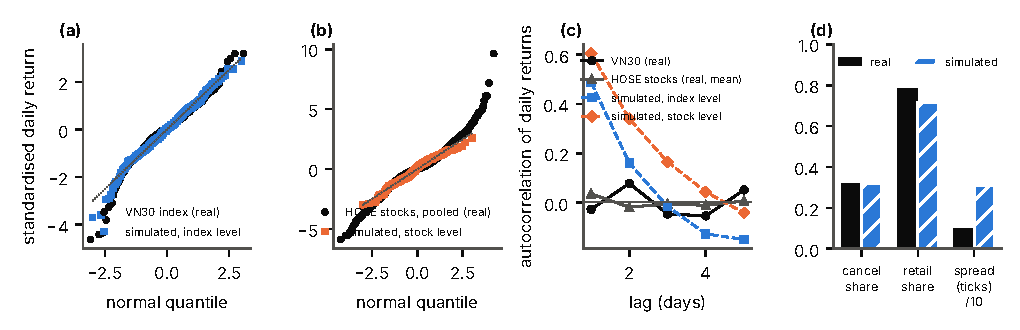
\includegraphics[width=\linewidth]{figures/calibration.pdf}
\caption{Calibration of the simulated markets against real data. (a) Standardised daily returns of the VN30 index since 2023 and of the first accepted index-level market, against normal quantiles. (b) Pooled standardised daily returns of 378 HOSE stocks since 2022 and of the first accepted stock-level market. (c) Autocorrelation of daily returns at lags 1 to 5: VN30 index, mean over HOSE stocks, and the first accepted market of each simulated family (pooled over episodes). (d) Cancel share, retail share (midpoint of the published range 0.75--0.82) and spread in ticks divided by 10 (VN30 futures: one tick for 73\% of quotes); the simulated spread is not matched}\label{fig:calibration}
\end{figure}


\section{A label-free screening statistic and its theory}\label{sec:method}

This section states the test, proves when it controls false alarms, gives a law for how its power depends on the number of accounts and on the size of a ring, shows why netting buys against sells protects against honest groups, and turns the power law into a deterrence condition for a regulator with a fixed inspection capacity. Section~\ref{sec:detect} checks every statement by simulation with the real implementation, and compares the power law with the agent-based market.

\subsection{The coincidence statistic}\label{sec:stat}

Take a window of $T$ steps and $N$ accounts. Let $x_i\in\mathbb R^T$ be account $i$'s signed submissions, $x_i[t]=$ buy orders minus sell orders submitted at step $t$, and let $y_{-i}=\sum_{j\ne i}x_j$ be the flow of all other accounts. For a tolerance $\tau\in\mathcal T$ let $\tilde y^{\tau}_{-i}[t]=\sum_{|d|\le\tau}y_{-i}[(t+d)\bmod T]$ (a circular box filter). For a shift $k\in\{0,\dots,T-1\}$ define the circular cross-correlation and the standardised statistic
\begin{equation}
C^{\tau}_i(k)=\sum_{t=0}^{T-1}x_i[(t-k)\bmod T]\;\tilde y^{\tau}_{-i}[t],\qquad
Z_i(k)=\max_{\tau\in\mathcal T}\frac{C^{\tau}_i(k)-\bar C^{\tau}_i}{s^{\tau}_i},
\label{eq:Z}
\end{equation}
where $\bar C^{\tau}_i$ and $s^{\tau}_i$ are the mean and standard deviation of $k\mapsto C^{\tau}_i(k)$ over the $T$ shifts. The statistic is large when account $i$ submits on the same side as the others at the same moments. The observed value is $Z_i(0)$; the circular-shift $p$-value is
\begin{equation}
p_i=\frac1T\,\#\{k\in\{0,\dots,T-1\}:\,Z_i(k)\ge Z_i(0)\}\in[1/T,1].
\label{eq:p}
\end{equation}
All $T$ shifts are computed by the fast Fourier transform, so one window costs $O(NT\log T)$ per tolerance; we use $T=300$ and $\mathcal T=\{1,5,15\}$. The \emph{unsigned} variant keeps buys and sells as two channels $x^{\mathrm b}_i,x^{\mathrm s}_i\ge0$ and adds their correlations before standardising. In use, the $B$ accounts with the largest $Z_i(0)$ in a window are inspected (``top-$B$''), or accounts with $p_i\le\alpha$ are flagged.

\subsection{Exact false-alarm control and its limits}\label{sec:valid}

\begin{proposition}[validity]\label{prop:exact}
Suppose that under the null hypothesis for account $i$ the pair $(x_i,y_{-i})$ is invariant in law to a cyclic shift of $x_i$ alone: $(g\,x_i,\,y_{-i})\overset{d}{=}(x_i,\,y_{-i})$ for every cyclic shift $g$. Then $\Pr(p_i\le\alpha)\le\alpha$ for every $\alpha\in[0,1]$.
\end{proposition}
\begin{proof}
Write $Z_k=Z_i(k)$ and $R_m=\#\{k:Z_k\ge Z_m\}$. Shifting $x_i$ by $g^j$ shifts the sequence $k\mapsto C^\tau_i(k)$ cyclically, so its mean and standard deviation over $k$ do not change, and $Z_k(x,y)=Z_0(g^kx,y)$. Hence $R_m(x,y)=R_0(g^mx,y)$ and by invariance $R_0\overset{d}{=}R_m$ for every $m$. For any real vector $(Z_k)$ and any $r>0$, at most $r$ indices $m$ satisfy $R_m\le r$: if $S$ is the set of such indices and $m^\ast\in S$ has the smallest $Z_{m^\ast}$, then every $m\in S$ has $Z_m\ge Z_{m^\ast}$, so $|S|\le R_{m^\ast}\le r$. Therefore $\Pr(R_0\le\alpha T)=\frac1T\sum_m\Pr(R_m\le\alpha T)=\frac1T\mathbb E\,\#\{m:R_m\le\alpha T\}\le\alpha$. \qedhere
\end{proof}

The maximum over tolerances is taken inside $Z_i(k)$ for the same $k$, so it does not break the argument. This is the standard randomisation-test argument \citep[see][for time-shift tests on dependent series]{liang2025}, and its condition is strong: it fails when account $i$ and the others share a trend or a burst inside the window, and when honest accounts react to the same event. Honest groups that act in step violate it; Section~\ref{sec:groups} shows how much and how netting removes most of it. Two consequences of the discreteness of $p_i$ matter for a regulator.

\begin{proposition}[inspection budget and resolution]\label{prop:budget}
Let $H$ be a set of accounts for which the condition of Proposition~\ref{prop:exact} holds, with arbitrary dependence between them. (a) For any $\alpha$, $\mathbb E\,\#\{i\in H:p_i\le\alpha\}\le |H|\alpha$; flagging at the threshold $\alpha=\lambda/N$ gives at most $\lambda$ expected false flags per window, and at most $\lambda W$ over $W$ windows. (b) Always $p_i\ge1/T$. Hence flagging with a family-wise error rate $\alpha_0$ by Bonferroni ($p_i\le\alpha_0/N$) is possible only if $T\ge N/\alpha_0$, that is for at most $N_{\max}=\alpha_0T$ accounts.
\end{proposition}
\begin{proof}
(a) is linearity of expectation applied to Proposition~\ref{prop:exact}; no independence is needed. (b) $p_i$ counts the shift $k=0$ itself. \qedhere
\end{proof}

With $T=300$ shifts and $\alpha_0=0.05$ the Bonferroni rule can handle only $15$ accounts, while a Vietnamese stock has hundreds of active accounts in a window of 300 minutes. Control with exact guarantees therefore needs either a finer resampling (more shifts than steps, as jitter surrogates provide) or ranking without a formal error bound. We use ranking (top-$B$), report the observed false-alarm rate, and treat the formal guarantee as per-account rather than per-family.

\subsection{Power: a law in the number of accounts and the size of the ring}\label{sec:power}

To see how detection depends on the market and on the ring, consider a Gaussian-flow model. Honest accounts have $x_i=e_i$ with $e_i[t]$ independent $\mathcal N(0,\sigma^2)$. A set of $k$ \emph{co-active} accounts (a ring, or the members that push together) each add the same signal, $x_i=e_i+b\,s$ for $i\le k$, with $s[t]\in\{0,1\}$ a campaign indicator and $\eta=b^2\mathrm{Var}(s)/\sigma^2$ the signal-to-noise ratio of one member.

\begin{proposition}[signal index]\label{prop:power}
In this model the population correlation between a co-active member's flow and the flow of all other accounts is
\begin{equation}
\rho_{N,k}(\eta)=\frac{(k-1)\,\eta}{\sqrt{(1+\eta)\,\bigl[(N-1)+(k-1)^2\eta\bigr]}},
\label{eq:rho}
\end{equation}
and an honest account has correlation $0$. For a single tolerance $\tau$ and a window of $T$ steps the statistic satisfies $Z_i(0)\approx\sqrt{T_{\mathrm{eff}}}\,\rho+\xi$ with $\xi$ standard normal, where $T_{\mathrm{eff}}\approx T/(2\tau+1)$ for white flows. Consequently: (i) $\rho$ increases in $k$ and in $\eta$ and saturates at $\sqrt{\eta/(1+\eta)}$ as $k\to\infty$; (ii) for $N\gg(k-1)^2\eta$, $\rho\approx(k-1)\eta/\sqrt{(1+\eta)N}$, so the shift of the statistic falls like $N^{-1/2}$; (iii) to keep a given power as $N$ grows the number of co-active accounts must grow like $\sqrt N$: the detectable size is $k-1\gtrsim(t+z_\beta)\sqrt{(1+\eta)N}/(\eta\sqrt{T_{\mathrm{eff}}})$, where $t$ is the critical value and $z_\beta$ the normal quantile of the target power.
\end{proposition}
\begin{proof}
Let $v_s=\mathrm{Var}(s)$. For a member $i$ and $y=y_{-i}$: $\mathrm{Cov}(x_i,y)=(k-1)b^2v_s=(k-1)\eta\sigma^2$, $\mathrm{Var}(x_i)=\sigma^2(1+\eta)$, and $\mathrm{Var}(y)=(N-1)\sigma^2+(k-1)^2b^2v_s=\sigma^2[(N-1)+(k-1)^2\eta]$, because the $N-1$ other noise terms are independent and the $k-1$ other members share the signal. Dividing gives~\eqref{eq:rho}. For honest $i$, $e_i$ is independent of $y$. Standardising $C(k)$ across shifts converts $T\,\widehat{\mathrm{cov}}(x_i,\tilde y)$ into $\sqrt T$ times the sample correlation when $x$ and $\tilde y$ are white, and a box filter of width $2\tau+1$ divides the effective number of independent samples by $2\tau+1$; the sample correlation is asymptotically $\mathcal N(\rho,1/T_{\mathrm{eff}})$ for small $\rho$. (i)--(iii) follow from~\eqref{eq:rho} by differentiation and by solving $\rho\sqrt{T_{\mathrm{eff}}}=t+z_\beta$. \qedhere
\end{proof}

Proposition~\ref{prop:power} is an approximation, not an exact result (the sample-correlation law is asymptotic and the maximum over tolerances adds a positive bias to $Z_i(0)$ in both hypotheses); Section~\ref{sec:powercheck} checks the linear dependence on $\rho$ and the $N^{-1/2}$ law in simulation. The predicted probability that a member is among the $B$ top-ranked accounts of $N$ follows from the null distribution $F_0$ of $Z_i(0)$: with $t_B=F_0^{-1}(1-B/N)$ and a mean shift $S=c\rho$,
\begin{equation}
q_B=1-F_0(t_B-S)\;\approx\;\Phi\!\bigl(S-\Phi^{-1}(1-B/N)\bigr),
\label{eq:qB}
\end{equation}
and a ring of $K$ accounts has a member among the top $B$ with probability about $1-(1-q_B)^K$ if members are treated as independent (they are positively dependent, so the approximation overstates detection at small $K$; Section~\ref{sec:powercheck} quantifies this).

\paragraph{Heterogeneous accounts.} If honest accounts have different noise variances $\sigma_j^2$ and member $i$ has $\sigma_i^2$, the same calculation gives $\rho$ as in~\eqref{eq:rho} with $\eta$ replaced by $\eta_i=b^2\mathrm{Var}(s)/\sigma_i^2$ and with $N-1$ replaced by the \emph{effective number of accounts} $N_{\mathrm{eff},i}=\sum_{j\ne i}\sigma_j^2/\sigma_i^2$, because $\mathrm{Var}(y_{-i})=\sum_{j\ne i}\sigma_j^2+(k-1)^2b^2\mathrm{Var}(s)$ and $\mathrm{Var}(x_i)=\sigma_i^2(1+\eta_i)$. A quiet account in a market whose aggregate flow is dominated by a few loud accounts therefore sees an $N_{\mathrm{eff}}$ far above the number of accounts, and its ring is correspondingly hard to see; Section~\ref{sec:real-accounts} measures $N_{\mathrm{eff}}\approx10^6$ against about 470 accounts on a real order flow.

\subsection{Honest groups and the netting of buys against sells}\label{sec:netting}

Market-making desks re-quote on both sides at the same moments. Suppose desk $i$ submits $b_i[t]=u[t]+\beta_i[t]$ buy and $s_i[t]=u[t]+\sigma_i[t]$ sell orders, where $u$ is the common re-quote activity and $\beta_i,\sigma_i$ are independent across accounts and sides.

\begin{proposition}[netting]\label{prop:netting}
For two desks $i\ne j$, the signed flows $x_i=b_i-s_i=\beta_i-\sigma_i$ and $x_j$ are uncorrelated at every lag, so their contribution to $\rho$ in~\eqref{eq:rho} is zero; the unsigned channels satisfy $\mathrm{Cov}(b_i+s_i,\;b_j+s_j)=4\,\mathrm{Var}(u)>0$. For a one-directional ring, $b_i=u+\beta_i$ and $s_i=\sigma_i$, the signed flows satisfy $\mathrm{Cov}(x_i,x_j)=\mathrm{Var}(u)$ and keep their signal, at the price of the extra variance $\mathrm{Var}(\sigma_i)$ in $x_i$.
\end{proposition}
\begin{proof}
$\mathrm{Cov}(\beta_i-\sigma_i,\beta_j-\sigma_j)=0$ by independence; $\mathrm{Cov}(u+\beta_i+u+\sigma_i,u+\beta_j+u+\sigma_j)=\mathrm{Var}(2u)=4\mathrm{Var}(u)$; and $\mathrm{Cov}(u+\beta_i-\sigma_i,u+\beta_j-\sigma_j)=\mathrm{Var}(u)$. \qedhere
\end{proof}

Netting therefore removes symmetric two-sided coordination at no cost to the test's validity, and costs power for a ring whose members also submit unrelated orders on the opposite side: the signal-to-noise ratio of the signed flow is lower than that of the buy channel alone by the factor $\mathrm{Var}(\beta_i+u)/\mathrm{Var}(\beta_i+u-\sigma_i)$. Section~\ref{sec:groups} measures both effects. Coordination that is two-sided in a way that does not cancel (for example a fund that buys at one moment in some accounts and sells in others) is not protected by netting.

\subsection{Deterrence with a fixed inspection capacity}\label{sec:deter}

Let a ring pick a strategy $\theta$ from a set $\Theta$, earn a random gross gain $g(\theta)$, and be \emph{caught} (event $D$) with probability $Q(\theta)$ if the regulator inspects the $B$ top-ranked accounts in each of $W$ windows; a caught ring pays $m\,g^+$ where $g^+=\max(g,0)$ and $m$ is the fine multiple (5 for individuals and 10 for organisations in Vietnam, Appendix~\ref{app:calib}). Its expected net benefit is
\begin{equation}
U(\theta)=\mathbb E[g]-m\,\mathbb E[g^+\mathbf 1_D].
\label{eq:U}
\end{equation}

\begin{proposition}[deterrence]\label{prop:deter}
If $D$ is independent of $g$ given $\theta$, then $U(\theta)=\mathbb E[g]-mQ\,\mathbb E[g^+]$, and $mQ\ge1$ implies $U(\theta)\le0$. If in addition $g\ge0$, then $U(\theta)\le0$ if and only if $Q\ge1/m$. In the screening model, with~\eqref{eq:qB} and members and windows treated as independent, $Q=1-\bigl(1-[1-(1-q_B)^K]\bigr)^W$ and the smallest capacity that deters a ring of $K$ accounts over $W$ windows at fine multiple $m$ is
\begin{equation}
B^\ast=N\,\Phi\!\bigl(\Phi^{-1}(q^\ast)-S\bigr),\qquad q^\ast=1-\bigl(1-r^\ast\bigr)^{1/K},\quad r^\ast=1-\bigl(1-1/m\bigr)^{1/W},
\label{eq:Bstar}
\end{equation}
whereas random inspection needs $B_{\mathrm{rand}}=Nq^\ast$. The saving $B_{\mathrm{rand}}/B^\ast=q^\ast/\Phi(\Phi^{-1}(q^\ast)-S)$ is at least $1$, increases in $S$, and tends to $1$ as $N\to\infty$ because $S\propto N^{-1/2}$.
\end{proposition}
\begin{proof}
$U=\mathbb E[g]-mQ\,\mathbb E[g^+]\le\mathbb E[g^+](1-mQ)\le0$ when $mQ\ge1$, since $\mathbb E[g]\le\mathbb E[g^+]$. If $g\ge0$ then $U=\mathbb E[g](1-mQ)$. The expression for $Q$ is the union over members and windows. Solving $Q=1/m$ for $q_B$ and inverting~\eqref{eq:qB} gives~\eqref{eq:Bstar}; the saving is the ratio of the two capacities, and $\Phi(z-S)\le\Phi(z)$ for $S\ge0$. \qedhere
\end{proof}

Two consequences are used in Section~\ref{sec:frontier}. First, a ring that is exposed in many windows by many accounts needs little capacity to be deterred, which is why adaptive rings shrink: they reduce $K$ and the number of active windows. Second, the advantage of screening over random inspection disappears in large markets unless the signal $S$ is boosted, for example by longer windows or better statistics; with $N=2000$ accounts and a ring of three the saving is less than a factor of two.

\subsection{A rule that changes the payoff: the block reference price}\label{sec:blocklaw}

In the simulator a ring holds a block before the campaign and sells it off-book at the end of each push at a \emph{reference price}, and the exchange can set the reference to the mean mid-price over the last $L$ steps ($L=1$ is the last price). The reference enters only the payoff, not the dynamics. Write $P_t$ for the mid-price and $\Delta P_t=P_t-P_{t-1}$.

\begin{proposition}[block reference price]\label{prop:block}
With $m_L(t)=\frac1L\sum_{s=0}^{L-1}P_{t-s}$, the price displacement credited to a block sold at the end $t$ of a push that began at mid-price $P_0$ is $D_L=D_1-\sum_{u=0}^{L-2}\bigl(1-\tfrac{u+1}{L}\bigr)\Delta P_{t-u}$, where $D_1=P_t-P_0$: only recent price increments count, discounted linearly with age. If the price rises linearly by $D_1$ over the last $a$ steps before the sale and is flat before, then
\begin{equation}
\frac{D_L}{D_1}=\begin{cases}\dfrac{a}{2L}, & L\ge a,\\[1ex] 1-\dfrac{L}{2a}, & L\le a.\end{cases}
\label{eq:blocklaw}
\end{equation}
If the ring instead holds the price at the top for $h$ further steps, $D_L/D_1=(a/2+h)/L$ for $L\ge a+h$, so keeping the full gain requires holding the price for about $L-a/2$ steps.
\end{proposition}
\begin{proof}
$P_t-m_L(t)=\frac1L\sum_{s=0}^{L-1}(P_t-P_{t-s})=\frac1L\sum_{s}\sum_{u<s}\Delta P_{t-u}=\sum_{u=0}^{L-2}\frac{L-1-u}{L}\Delta P_{t-u}$ and $D_L=(m_L(t)-P_0)=D_1-(P_t-m_L(t))$. For the ramp, the average of the last $L$ prices above $P_0$ is $D_1a/(2L)$ when $L\ge a$ (the ramp has mean $D_1/2$ over $a$ of the $L$ steps) and $D_1(1-L/(2a))$ when $L\le a$; holding adds $h$ steps at $D_1$. \qedhere
\end{proof}

The rule therefore replaces the price level by an exponentially-flat memory of the path: a one-day reference ($L=240$) pays a ring that pushes for $a\approx60$ steps a quarter of what the last price pays, and the ring can recover the gain only by holding the price, which is the manipulation the rule penalises. Because the rule changes the payoff only, its effect on a ring that does not adapt can be computed exactly from the same simulated episodes for every $L$, and compared with the best response; this is done in Section~\ref{sec:blockcheck}.

\subsection{Evaluating a rule by the ring's best response}\label{sec:br}

Let $\pi\in\Pi$ be a policy (band, block reference $L$, inspection capacity $B$, order-level rules), $\varphi$ a market in a family $\mathcal M$, and $U(\theta;\pi,\varphi)$ the ring's net benefit~\eqref{eq:U}. The ring's value is $V(\pi;\varphi)=\sup_{\theta\in\Theta}U(\theta;\pi,\varphi)$. The regulator compares policies by the distribution of $V(\pi;\varphi)$ over $\varphi\in\mathcal M$ together with the cost to honest participants $C(\pi;\varphi)$ (spread, depth, volatility); it deems $\pi$ \emph{deterring} in $\varphi$ if $V(\pi;\varphi)\le0$.

\begin{proposition}[best response on a finite strategy set]\label{prop:lower}
Let $\hat\Theta\subset\Theta$ be finite, let $\hat\theta$ maximise the mean over $n$ selection episodes, and let $\hat U$ be the mean over $n$ further, independent episodes. Then $\mathbb E[\hat U\mid\hat\theta]=U(\hat\theta;\pi,\varphi)\le V(\pi;\varphi)$. Hence the reported ring benefit is unbiased for the benefit of the chosen strategy and a lower bound in expectation of the true best response, and a policy that appears deterring on $\hat\Theta$ may not be deterring against a larger set.
\end{proposition}
\begin{proof}
$\hat U$ is independent of $\hat\theta$ given the market, so conditioning removes the selection bias; and $U(\hat\theta)\le\sup_\Theta U$. \qedhere
\end{proof}

The proposition is the reason for the statements throughout that the effects of rules on rings are conservative for the ring: with a better search, rings would do at least as well, and deterrence results are upper bounds on what a regulator can claim. The family $\mathcal M$ is drawn by approximate Bayesian rejection: parameters of the honest market are sampled, honest-only episodes are simulated, and a draw is kept if its cancel share, retail share and daily volatility are within tolerance of the real values (Section~\ref{sec:calib}). A conclusion that holds for every accepted market is more credible than one tuned to a single calibration, but the tolerance box is wide, and markets that match the moments need not match anything else.


\section{Experiments I: the screening statistic}\label{sec:detect}

We check the statements of Section~\ref{sec:method} on the test in three steps (the deterrence and block-price laws are checked in Section~\ref{sec:policy}): with synthetic flows where the truth is known (validity, budget, power law, netting), in the agent-based market with a ring and honest groups (sensitivity, robustness, comparison with other detectors), and on real account-level order flow (Section~\ref{sec:real-accounts}). Unless stated, the agent-based results are for the default simulator (100 to 170 accounts in a window), one ring per episode, episodes of 6000 steps (19 windows of 300 steps), and the metric is \emph{catch@$B$}: the share of ring-active windows in which one of the $B$ top-ranked accounts is a ring member, with 95\% bootstrap intervals over 24 test episodes.

\subsection{Validity and the inspection budget (Propositions~\ref{prop:exact} and~\ref{prop:budget})}\label{sec:validcheck}

Figure~\ref{fig:theory}a gives the rejection rate of the implemented signed test against its nominal level for exchangeable flows. For independent Gaussian flows and for Poisson counts the rate is at the nominal level (0.0100 and 0.0102 at the 1\% level, 0.051 and 0.052 at 5\%, 18,000 tests each). Rejection is zero at the 0.1\% level because $p\ge1/T=1/300$ (Proposition~\ref{prop:budget}b). The condition of the proposition is violated by flows with a shared regime, bursts of activity that all accounts follow: the unsigned test then rejects 65\% of honest accounts at the 1\% level, and the signed test, in which symmetric bursts cancel, 1.5\%. Figure~\ref{fig:theory}b confirms the expected number of honest flags per window against the bound $N\alpha$ for $N$ from 50 to 1200, and the Bonferroni rule at level 5\% flags nothing for any of these $N$, as the resolution limit says. We therefore use the test as a ranking device and report observed rates.

\begin{figure}[t]
\centering
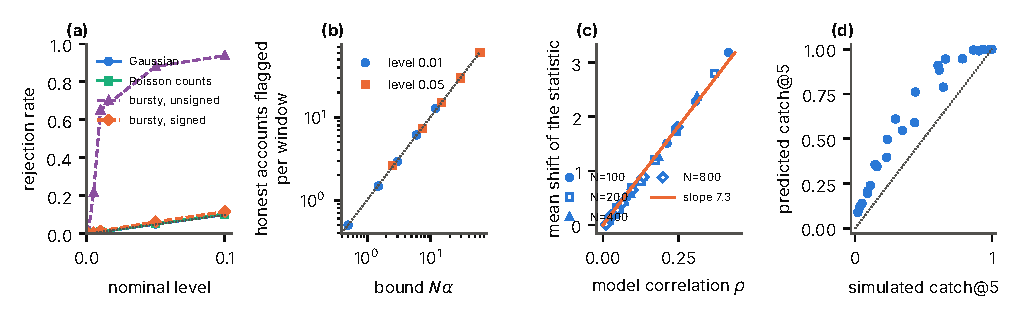
\includegraphics[width=\linewidth]{figures/theory.pdf}
\caption{Monte Carlo checks of the propositions with the implemented test. (a) Rejection rate against nominal level for exchangeable flows (Gaussian, Poisson) and for flows with a shared bursty regime (signed and unsigned variants); dotted line: nominal. (b) Honest accounts flagged per window against the bound $N\alpha$ at levels 1\% and 5\%. (c) Mean shift of a ring member's statistic against the model correlation $\rho$ of Proposition~\ref{prop:power}, for $N$ from 100 to 800, $k$ from 4 to 32 and $\eta\in\{0.1,0.3\}$; line: fitted slope. (d) Predicted against simulated catch@5 for the same 32 settings}\label{fig:theory}
\end{figure}

\subsection{The power law (Proposition~\ref{prop:power})}\label{sec:powercheck}

In a Gaussian-flow market with $N$ from 100 to 800 accounts, ring sizes from 4 to 32 and signal-to-noise ratios $\eta\in\{0.1,0.3\}$ (32 settings, 200 windows each), the mean shift of a member's statistic over the honest mean is linear in the model correlation $\rho$ of~\eqref{eq:rho} (Figure~\ref{fig:theory}c; through the origin, $R^2=0.993$; fitted slope $\sqrt{T_{\mathrm{eff}}}=7.3$, that is $T_{\mathrm{eff}}\approx53$ of $T=300$, within a factor of two of $T/(2\tau+1)=100$ for the smallest tolerance). The predicted catch@5 from~\eqref{eq:qB}, with members treated as independent, tracks the simulated one (correlation 0.96) but overstates it by 0.13 on average (Figure~\ref{fig:theory}d), because members' statistics are positively dependent through the shared signal and the shared aggregate. The law is therefore a good guide to \emph{how} detection varies with $N$ and $k$ and a poor guide to its level at small $k$.

In the agent-based market the same law explains the dependence on the number of accounts. The ring there has structure the Gaussian model omits: only the $m_{\mathrm{push}}$ members that push together are co-active, so the number of co-active accounts does not change with the ring size $K$, and the signal is proportional to the push probability. The model fitted to the three one-factor sweeps is
\begin{equation}
\text{shift}=s_0\,\frac{p_{\mathrm{push}}}{0.8}\Bigl(\frac{100}{N}\Bigr)^{1/2},\qquad
\text{catch@}B=a\,\bigl[1-(1-q_B)^K\bigr],
\label{eq:fit}
\end{equation}
with $q_B$ from~\eqref{eq:qB}, two constants ($s_0=1.20$ standard units of the statistic at $N=100$, and a ceiling $a=0.90$ for ring-active windows without signal) and the exponent $1/2$ taken from the theory. The 11 points are fitted with a mean absolute error of 0.043 (Figure~\ref{fig:powerabm}); holding one sweep out and predicting it from the other two gives errors of 0.045 for ring size, 0.085 for the number of accounts (where the $N^{-1/2}$ law is a pure prediction) and 0.088 for the push probability. When the exponent is left free it is $0.32$, below the theoretical $0.5$; with 11 points we cannot say whether this reflects the non-Gaussian flows or noise, but both give detection falling steeply with $N$: catch@5 is 0.91 at 100 accounts and 0.28 at 708.

\begin{figure}[t]
\centering
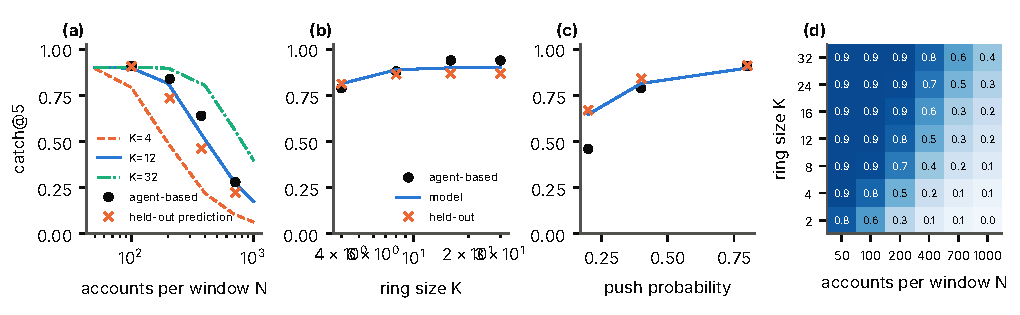
\includegraphics[width=\linewidth]{figures/power_abm.pdf}
\caption{The scaling law against the agent-based market. (a)--(c) catch@5 against the number of accounts, the ring size and the push probability: points are simulated, lines are the model~\eqref{eq:fit} fitted to all sweeps, crosses are predictions with the plotted sweep held out. (d) Model catch@5 over the number of accounts and the ring size at push probability 0.8}\label{fig:powerabm}
\end{figure}

\subsection{Honest groups and netting (Proposition~\ref{prop:netting})}\label{sec:groups}

With synthetic flows, six market-making-like desks that re-quote on both sides at the same moments are flagged at the 1\% level in 80\% of cases by the unsigned test and in 1.1\% by the signed test, whereas a one-directional ring is flagged in 37\% by the unsigned and 17\% by the signed test: netting removes the desks and costs power for the ring, as the proposition says. In the agent-based market, Table~\ref{tab:robust} and Figure~\ref{fig:robust} give catch@5 with and without honest groups. The baselines that need no labels fail on the ring: the order-to-trade ratio is dominated by market makers, which sit far above manipulators, and an isolation forest on account features finds almost nothing. The unsigned test finds the ring in a clean market but collapses when market-making desks are present, because the desks are flagged at 71\% (Table~\ref{tab:groups}) and fill the top of the ranking. Netting buys against sells removes the effect of the desks (their flag rate falls to 0 in that scenario and catch@5 stays at 0.88). A fund that splits orders across sub-accounts is genuinely coordinated and is flagged at 6\% whatever the variant; it reduces catch@5 to 0.74. With all three honest groups together catch@5 is 0.52 for the signed test and 0.23 for the unsigned one, and the desks are flagged at 18\% even after netting. A gradient-boosting model trained with labels on rings in the clean market stays at 0.98--1.00 in every scenario.

\begin{figure}[t]
\centering
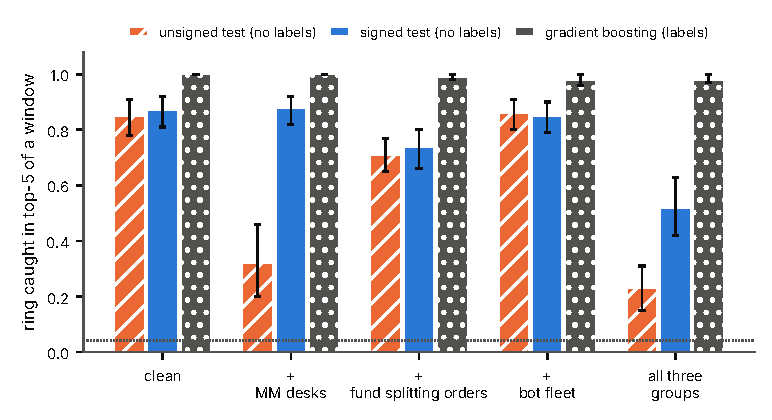
\includegraphics[width=0.85\linewidth]{figures/robust.pdf}
\caption{Share of ring-active windows in which a ring member is among the five top-ranked accounts, with 95\% bootstrap intervals over 24 episodes. The dotted line is the chance level. The unsigned test is crowded out by market-making desks; the signed test is not. Gradient boosting is trained with labels on rings in the clean market}\label{fig:robust}
\end{figure}

\begin{table}[t]
\centering\footnotesize
\adjustbox{max width=\linewidth}{\begin{tabular}{lccccc}
\toprule
detector & clean & +MM desks & +fund splitting orders & +bot fleet & all three \\
\midrule
order-to-trade ratio & 0.00\,{\scriptsize[0.00, 0.00]} & 0.00\,{\scriptsize[0.00, 0.00]} & 0.00\,{\scriptsize[0.00, 0.00]} & 0.13\,{\scriptsize[0.05, 0.22]} & 0.09\,{\scriptsize[0.04, 0.14]} \\
isolation forest (no labels) & 0.01\,{\scriptsize[0.00, 0.02]} & 0.01\,{\scriptsize[0.00, 0.02]} & 0.00\,{\scriptsize[0.00, 0.00]} & 0.01\,{\scriptsize[0.00, 0.03]} & 0.02\,{\scriptsize[0.00, 0.03]} \\
coincidence test, unsigned (no labels) & 0.85\,{\scriptsize[0.78, 0.91]} & 0.32\,{\scriptsize[0.20, 0.46]} & 0.71\,{\scriptsize[0.65, 0.77]} & 0.86\,{\scriptsize[0.80, 0.91]} & 0.23\,{\scriptsize[0.15, 0.31]} \\
coincidence test, signed (no labels) & 0.87\,{\scriptsize[0.81, 0.92]} & 0.88\,{\scriptsize[0.82, 0.92]} & 0.74\,{\scriptsize[0.66, 0.80]} & 0.85\,{\scriptsize[0.79, 0.90]} & 0.52\,{\scriptsize[0.42, 0.63]} \\
gradient boosting (labels, clean market) & 1.00\,{\scriptsize[1.00, 1.00]} & 1.00\,{\scriptsize[1.00, 1.00]} & 0.99\,{\scriptsize[0.98, 1.00]} & 0.98\,{\scriptsize[0.96, 1.00]} & 0.98\,{\scriptsize[0.97, 1.00]} \\
\bottomrule
\end{tabular}
}
\caption{catch@5 in a clean market and with honest groups acting in step (95\% bootstrap intervals).}\label{tab:robust}
\end{table}

\begin{table}[t]
\centering\footnotesize
\begin{adjustbox}{max width=\linewidth}
\begin{tabular}{llrrr}
\toprule
scenario & honest group & members scored & flagged, unsigned & flagged, signed\\
\midrule
+ market-making desks & market-making desks & 2622 & 0.711 & 0.000\\
+ fund splitting orders & fund sub-accounts & 5277 & 0.061 & 0.063\\
+ bot fleet & bot fleet & 3571 & 0.013 & 0.016\\
all three & market-making desks & 2698 & 0.665 & 0.182\\
all three & fund sub-accounts & 5202 & 0.050 & 0.053\\
all three & bot fleet & 3732 & 0.029 & 0.037\\
\bottomrule
\end{tabular}
\end{adjustbox}
\caption{Honest group members flagged at $p\le 0.01$ (nominal 1\%).}\label{tab:groups}
\end{table}

\subsection{Comparison with other detectors}\label{sec:roc}

Figure~\ref{fig:roc} gives receiver-operating and precision--recall curves of the account-window scores for the unsigned and signed tests, the supervised model and an isolation forest, in the clean market, with market-making desks and with all three honest groups. The signed test has an area under the curve of 0.85, 0.87 and 0.73 in the three scenarios and the unsigned test 0.84, 0.79 and 0.72; the supervised model 0.99, 0.99 and 0.98; the isolation forest and the order-to-trade ratio are below chance (0.36 to 0.46): the order-to-trade ratio is dominated by market makers, and the most unusual accounts by their features are not the ring members. The average precision of the label-free tests is low, 0.24, 0.27 and 0.075 for the signed test (0.22, 0.10 and 0.06 unsigned) against 0.89 to 0.94 for the supervised model and a share of 3\% to 4\% of ring members among the account-windows. The label-free tests are informative over the whole ranking but their precision is high only at its very top, which is what catch@5 measures; they are not a classifier. The netting in the signed test matters most with market-making desks (average precision 0.27 against 0.10).

\begin{figure}[t]
\centering
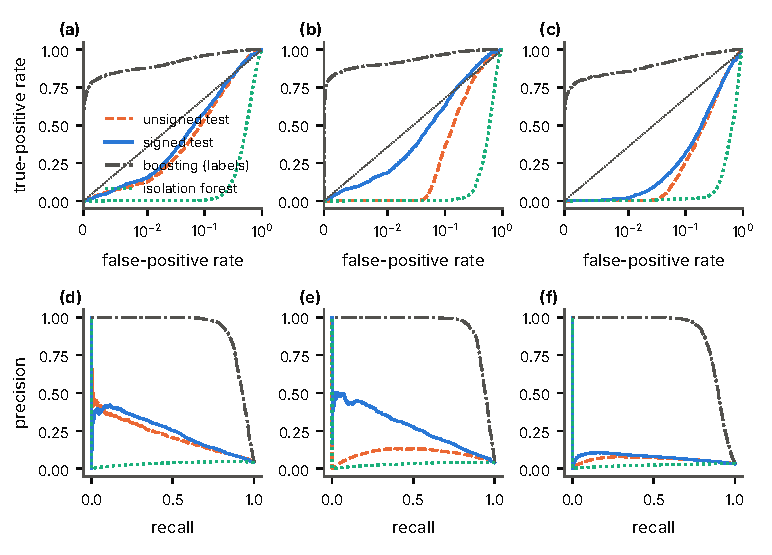
\includegraphics[width=\linewidth]{figures/roc.pdf}
\caption{Receiver-operating (top) and precision--recall (bottom) curves of account-window scores for ring membership, in a clean market (a, d), with market-making desks (b, e) and with all three honest groups (c, f); 24 test episodes each. The supervised model is trained with labels in the clean market only}\label{fig:roc}
\end{figure}

\subsection{Sensitivity}\label{sec:sens}

Figure~\ref{fig:sens} and the ablation table of Appendix~\ref{app:extra} vary the design. The tolerance set and the window length matter little (catch@5 between 0.88 and 0.91). Sensitivity falls with the number of accounts and rises with ring size (0.79 for four accounts, 0.94 for 16 or more) and with the ring's activity (0.46, 0.79, 0.91 for push probabilities 0.2, 0.4, 0.8), as the law predicts (Figure~\ref{fig:powerabm}). The dependence on the number of accounts is the main weakness of ranking by top-$B$; a rule based on finer resampling and a false-discovery-rate bound would scale differently, and we have not tested it.

\begin{figure}[t]
\centering
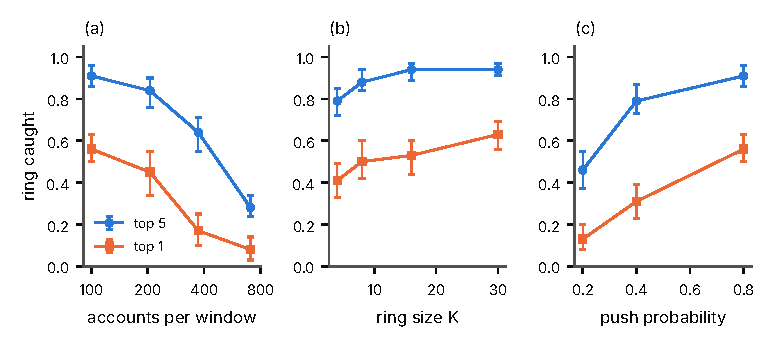
\includegraphics[width=\linewidth]{figures/sensitivity.pdf}
\caption{Sensitivity of the signed test in a clean market: (a) number of accounts per window, (b) ring size, (c) push probability of the ring. Bars are 95\% bootstrap intervals over 16 episodes}\label{fig:sens}
\end{figure}

\paragraph{What the label-free test is for.} The model trained with labels is better in every simulated scenario. The label-free test is useful when there are no labels, which is the regulator's position, and when one cannot trust that a model trained on simulated rings transfers to real ones. Section~\ref{sec:real-accounts} shows that the second concern is justified for the test itself: on real order flow it also faces a background the simulator does not contain.


\section{Experiments II: rules against a ring that adapts}\label{sec:policy}

\subsection{Design}

\paragraph{Levers.} The daily price band ($7\%$ today, $10\%$, $15\%$ or none); the reference price of off-book block trades (the last price, or the mean over the last $L=60$ or $240$ steps); inspection of the $B$ top-ranked accounts per window by the signed test, with a fine of $m$ times the illegal gain; a minimum resting time before an order may be cancelled (5 or 15 steps); a fee per cancelled order; a larger tick; a circuit breaker. With $m=5$ and $m=10$, deterrence needs a probability of detection above $1/m$ (Proposition~\ref{prop:deter}).

\paragraph{Manipulators.} The ring chooses a strategy from the 11-parameter space of Table~\ref{tab:space}. Because single evolution-strategy runs were noisy and non-monotone across policies, every policy faces the same set of four ring strategies (the strongest found under different policies in one market, the default ring, and the strongest unconstrained one); the ring picks the best on 12 selection episodes and the tables report 12 separate episodes (Proposition~\ref{prop:lower}: a lower bound on a fully adaptive ring). The spoofer, the pump-and-dump agent and the wash pair use fixed strategies and are evaluated for what they achieve; for them the effect of a rule is an upper bound.

\paragraph{Families of markets.} Market parameters (numbers of noise and fundamental traders, market-maker activity and sensitivity to displayed depth, volatility of the latent value, momentum activity) are drawn at random, honest-only markets are simulated, and a draw is kept if its cancel share (0.27--0.37), retail share (0.66--0.85) and daily volatility (0.9--1.4\% for the index-level family, 1.8--2.8\% for the stock-level family) are within tolerance of the real ones, an approximate Bayesian rejection. We keep six markets per family (6 of 27 draws and 6 of 62 draws) and report the distribution of each outcome over markets. Acceptance used only two episodes per draw, so it is noisy: re-measured over 16 episodes (Appendix~\ref{app:extra}), the volatility is inside the tolerance in five of six index-level and four of six stock-level markets, the cancel share in five of six in each family and the retail share in all, and the excursions are of one to two standard errors of the re-measurement. Figure~\ref{fig:calibration} compares the first accepted markets with real returns.

\subsection{The ring against each rule}

Figure~\ref{fig:ensemble} and Table~\ref{tab:ensemble} give the ring's gain in the index-level family. The daily price band does not change the ring's gain (median ratio to no policy $0.97$; the ring moves the price by about 0.5\%, far inside a band of 7\%), and widening it to 10\% or 15\%, which the securities commission is studying, changes nothing in the single market where we tried it (Appendix~\ref{app:single}). Pricing blocks at the trailing mean cuts the gain, Section~\ref{sec:blockcheck} analyses how much. Inspection deters the ring only with enough capacity: with three inspected accounts per window (0.5\% of accounts) the ring's expected net benefit at $m=5$ is non-positive in five of six markets, with one inspected account in two of six; the median probability of being caught is 42\% and 17\%.

\begin{figure}[t]
\centering
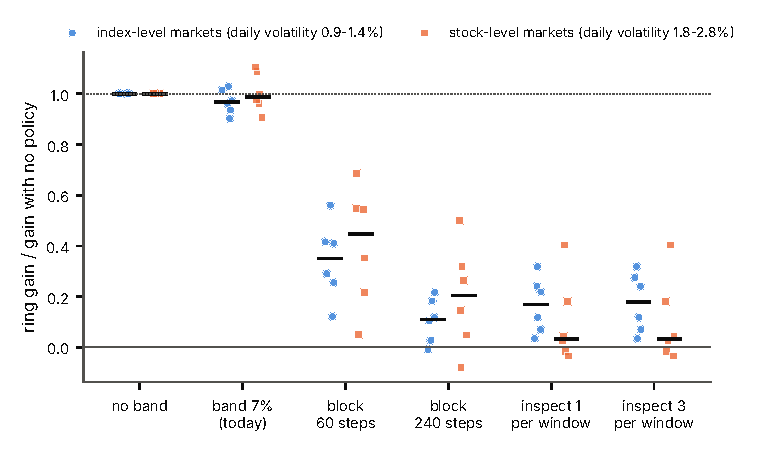
\includegraphics[width=0.95\linewidth]{figures/ensemble.pdf}
\caption{The best-responding ring's gain relative to its gain with no policy, one point per calibrated market and the median as a line. Daily band 7\% in all policies but the first}\label{fig:ensemble}
\end{figure}

\begin{table}[t]
\centering\footnotesize
\adjustbox{max width=\linewidth}{\begin{tabular}{lrrrrr}
\toprule
policy & median gain & range over markets & median ratio to no policy & median detection prob. & deterred at $m=5$ \\
\midrule
no price band & 110.0k & 86.7k to 162.1k & 1.00 & -- & -- \\
band 7\% (HOSE today) & 105.0k & 89.2k to 164.6k & 0.97 & -- & -- \\
band 7\% + block at 60-step mean & 38.4k & 11.7k to 90.8k & 0.35 & -- & -- \\
band 7\% + block at 240-step mean & 15.3k & -0.9k to 23.5k & 0.11 & -- & -- \\
band 7\% + inspect 1 per window & 16.8k & 4.5k to 51.6k & 0.17 & 17\% & 2/6 \\
band 7\% + inspect 3 per window & 16.8k & 4.5k to 51.6k & 0.18 & 42\% & 5/6 \\
\bottomrule
\end{tabular}
}
\caption{Index-level family of six calibrated markets: the best-responding ring's gain (tick-lots) against each policy, the median probability that a member is inspected in some window of an episode, and the number of markets in which the ring's expected net benefit is non-positive at a fine of five times the gain.}\label{tab:ensemble}
\end{table}

\paragraph{Stock-level family.} The case stocks are more volatile than the index, so we repeat the exercise with six markets whose daily volatility is 1.8--2.8\% (Table~\ref{tab:ensemblestock}; same ring strategy set, not re-optimised). The ring's gain with no policy is larger (median 164k against 110k at index level). The conclusions on the band and on inspection are unchanged in sign: the band leaves the gain at a median 99\% of its value. Under inspection the best-responding ring shrinks its operation: its median gain falls to 3\% of the no-policy gain (6k), with a median probability of being caught of 8\% with one inspected account per window and 25\% with three. The ring's expected net benefit at $m=5$ is non-positive in three of six markets with one inspected account and in five of six with three; in the remaining market with one inspected account the ring still nets up to 41k, and with three up to 7k. The detection probabilities are lower than at index level, where each window has fewer accounts to cover, yet deterrence is not worse, because the ring's remaining gain is smaller relative to the fine; we have not separated the two effects. In both families the price band has no effect, block pricing and inspection have large ones, and no single rule removes the ring's gain in every market.

\begin{table}[t]
\centering\footnotesize
\adjustbox{max width=\linewidth}{\begin{tabular}{lrrrrr}
\toprule
policy & median gain & range over markets & median ratio to no policy & median detection prob. & deterred at $m=5$ \\
\midrule
no price band & 164.4k & 101.2k to 261.4k & 1.00 & -- & -- \\
band 7\% (HOSE today) & 154.9k & 111.9k to 261.1k & 0.99 & -- & -- \\
band 7\% + block at 60-step mean & 66.5k & 8.4k to 179.0k & 0.45 & -- & -- \\
band 7\% + block at 240-step mean & 33.7k & -7.9k to 131.0k & 0.20 & -- & -- \\
band 7\% + inspect 1 per window & 6.3k & -9.1k to 40.8k & 0.03 & 8\% & 3/6 \\
band 7\% + inspect 3 per window & 6.3k & -9.1k to 40.8k & 0.03 & 25\% & 5/6 \\
\bottomrule
\end{tabular}
}
\caption{Stock-level family of six calibrated markets (daily volatility 1.8--2.8\%): the ring's gain against each policy, as in Table~\ref{tab:ensemble}.}\label{tab:ensemblestock}
\end{table}

\subsection{Markets without trending}\label{sec:acf}

\textit{(pending)}

\subsection{The block reference price: law, ex-post evaluation and best response}\label{sec:blockcheck}

Because the reference price enters only the ring's payoff (Section~\ref{sec:blocklaw}), the effect of the rule for every $L$ can be computed exactly from the same simulated episodes. For each market of both families and each of the four strategies we simulate 12 selection and 12 reporting episodes once and score them with $L\in\{1,5,15,30,60,120,240,480\}$. Table~\ref{tab:block} and Figure~\ref{fig:block} report the median over markets. The \emph{block term} is the value of the block alone (block size times credited displacement); the total gain adds trading profit, which the rule does not touch. The rule removes most of the block term: a reference of 60 steps leaves 42\% (index level) and 39\% (stock level) of it, a one-day reference 13\% and 2\%. The linear-ramp law of Proposition~\ref{prop:block}, with the measured push duration $a=72$ to $83$ steps, has the right shape and order of magnitude but overstates the retained value at $L\ge30$ (0.61 against 0.42 at $L=60$ at index level, 0.16 against 0.13 at $L=240$), because the real price path is not a ramp ending at the sale. The total gain falls to a median 52\% (60 steps) and 28\% (240 steps) of its value at index level and to 69\% and 44\% at stock level, as the trading profit remains; with a reference of two days ($L=480$) the median total gain is about zero ($-0.03$ at index level, $0.12$ at stock level), and in markets where the unconstrained gain is small the ring loses money already at 60 to 240 steps. Re-selecting the strategy (``adaptive'') changes the median only slightly: within the four strategies the ring finds no good counter, and the gap between the adaptive and the static curve is the value of adaptation. The independent episodes of the earlier ensemble run (Table~\ref{tab:ensemble}) give a lower retained share of the total gain (35\% and 11\% at index level, 45\% and 20\% at stock level for 60 and 240 steps); with episode-to-episode standard errors of about a third of the mean in gain, we read the evidence as: a one-day reference leaves the ring between roughly one tenth and one half of its gain, and removes most of the block value.

\paragraph{Sensitivity to the block size.} The block of 3000 lots is an assumption of the simulator, and it matters: the rule acts on the block term only, so its effect on the total gain depends on how much of the gain comes from the block. The size enters only the payoff, so a different size can be evaluated exactly on the same episodes (Appendix~\ref{app:extra}). With a block of 10,000 lots the ring keeps 19--21\% of its gain at a one-day reference; with the assumed size 28--44\%; with a block of 1000 lots 60--64\%, and of 300 lots 83--87\%, because trading profit then dominates. The rule is effective against a ring whose gain is realised through off-book blocks and has no effect on a ring that profits through trading on the book.

\begin{figure}[t]
\centering
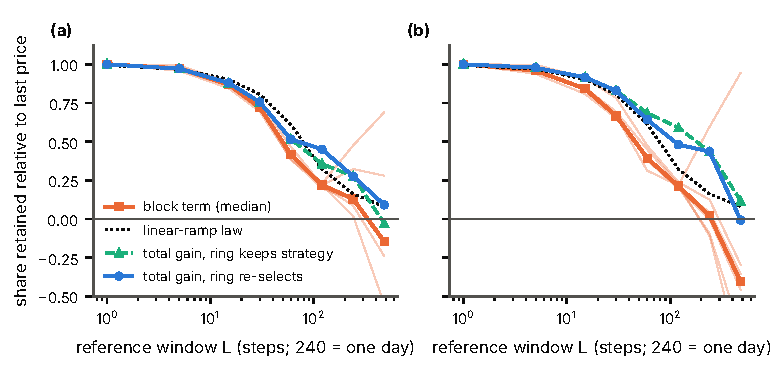
\includegraphics[width=\linewidth]{figures/block.pdf}
\caption{Share of the ring's block term and of its total gain retained against the reference window $L$, for the index-level (a) and stock-level (b) families: median over six markets of the block term (thick orange; thin lines are the six markets), the linear-ramp law of Proposition~\ref{prop:block}, and the total gain for a ring that keeps its strategy and for a ring that re-selects it}\label{fig:block}
\end{figure}

\begin{table}[t]
\centering\scriptsize
\setlength{\tabcolsep}{3pt}
\adjustbox{max width=\linewidth}{\begin{tabular}{lrrrrrrrr}
\toprule
& \multicolumn{4}{c}{index level} & \multicolumn{4}{c}{stock level} \\
\cmidrule(lr){2-5}\cmidrule(lr){6-9}
$L$ & block term & law & total, static & total, adaptive & block term & law & total, static & total, adaptive \\
\midrule
15 & 0.87 & 0.90 & 0.88 & 0.88 & 0.84 & 0.90 & 0.91 & 0.91 \\
30 & 0.72 & 0.81 & 0.76 & 0.76 & 0.67 & 0.81 & 0.83 & 0.83 \\
60 & 0.42 & 0.61 & 0.52 & 0.52 & 0.39 & 0.61 & 0.68 & 0.64 \\
120 & 0.22 & 0.32 & 0.36 & 0.45 & 0.21 & 0.32 & 0.59 & 0.48 \\
240 & 0.13 & 0.16 & 0.28 & 0.28 & 0.02 & 0.16 & 0.44 & 0.44 \\
480 & -0.15 & 0.08 & -0.03 & 0.09 & -0.41 & 0.08 & 0.12 & -0.01 \\
\bottomrule
\end{tabular}
}
\caption{Block-price rule, median over six markets per family: share of the block term and of the total gain retained when the block is priced at the mean of the last $L$ steps instead of the last price, and the prediction of the linear-ramp law.}\label{tab:block}
\end{table}

\subsection{Inspection capacity and the deterrence frontier}\label{sec:frontier}

Proposition~\ref{prop:deter} turns the power law into a capacity requirement. With the constants fitted in Section~\ref{sec:powercheck} ($s_0=1.20$), Table~\ref{tab:capacity} gives the number of accounts that must be inspected per window to deter a ring of three accounts active in four windows, and the saving over random inspection. In a market with 600 active accounts per window, screening deters at a fine of five times the gain with about 3 inspected accounts per window (0.5\% of accounts) against 11 for random inspection, and at ten times with 1.2 against 5.2; doubling the fine multiple therefore saves a factor of about 2.4 in capacity, which gives the regulator two exchangeable instruments (Section~\ref{sec:discussion}). The advantage of screening shrinks as the market grows (saving of 3.7 at 600 accounts and 2.0 at 2000). The model's detection probability for a ring of three accounts in four windows with one and three inspected accounts (8\% and 20\%) is close to the probability found for the best-responding ring in the stock-level family (8\% and 25\%) and below that of the index-level family (17\% and 42\%; Figure~\ref{fig:frontier}a). We do not know which sizes the best-responding ring chose, so this agreement is suggestive, not a test.

\begin{figure}[t]
\centering
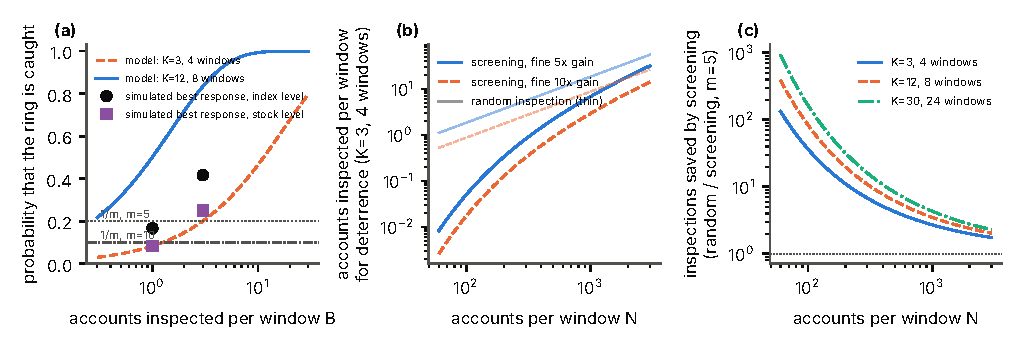
\includegraphics[width=\linewidth]{figures/frontier.pdf}
\caption{Deterrence frontier. (a) Probability that the ring is caught against the number of inspected accounts per window at $N=600$ for two ring sizes (model, solid and dashed), with the thresholds $1/m$ for $m=5,10$ (horizontal lines) and the median probability of the best-responding ring in the two simulated families (points). (b) Accounts to inspect per window for deterrence of a ring of three accounts active in four windows against $N$, by screening (thick) and by random inspection (thin). (c) Inspections saved by screening against $N$ for three ring sizes and activity levels, fine five times the gain}\label{fig:frontier}
\end{figure}

\begin{table}[t]
\centering\footnotesize
\adjustbox{max width=\linewidth}{\begin{tabular}{lrrrrrr}
\toprule
& \multicolumn{3}{c}{fine $5\times$ gain} & \multicolumn{3}{c}{fine $10\times$ gain} \\
\cmidrule(lr){2-4}\cmidrule(lr){5-7}
$N$ & screening & random & saving & screening & random & saving \\
\midrule
100 & 0.05 & 1.8 & 36.5 & 0.02 & 0.9 & 50.2 \\
300 & 0.81 & 5.5 & 6.8 & 0.32 & 2.6 & 8.1 \\
600 & 2.99 & 11.1 & 3.7 & 1.25 & 5.2 & 4.2 \\
1000 & 6.81 & 18.4 & 2.7 & 2.93 & 8.7 & 3.0 \\
2000 & 18.48 & 36.8 & 2.0 & 8.17 & 17.5 & 2.1 \\
\bottomrule
\end{tabular}
}
\caption{Inspected accounts per window needed to deter a ring of three accounts active in four windows (Proposition~\ref{prop:deter} with $s_0=1.20$): by screening and by random inspection, and the saving, for fine multiples 5 and 10.}\label{tab:capacity}
\end{table}

\subsection{Other manipulation types and the cost to honest investors}

Table~\ref{tab:matrix} and Figure~\ref{fig:tradeoff} report, for the first calibrated market, what a fixed spoofer, pump-and-dump agent, wash pair and ring achieve under order-level rules and what the rules cost honest participants. In this market, minimum resting times and cancel fees do not reduce what the manipulators achieve: spoofing profit is 872 (s.e.\ 125) with no rule and 1,091 to 1,380 with minimum resting times or fees, and the spoofing price impact is higher, not lower, with a longer minimum resting time (0.26 against 0.11 ticks); pump impact is lower under cancel fees (0.31 against 0.47, within about 1.3 standard errors); wash volume is 3.3\% of volume under every rule, and the ring's gain is unaffected except by the block price. These rules cost honest investors: a minimum resting time of 15 steps raises the spread by 7\% and volatility by 21\%, and a cancel fee of 2 raises volatility by 24\%. A tick twice as large widens the spread by 35\% and cuts depth by 10\% while lowering spoofing profit (491 against 872). The block price rule has no effect on honest trading in this experiment because honest agents do not trade blocks; its cost is the gap between the last price and the trailing mean, 0.17\% of price at 60 steps and 0.50\% at 240 steps in the first preset.

\begin{figure}[t]
\centering
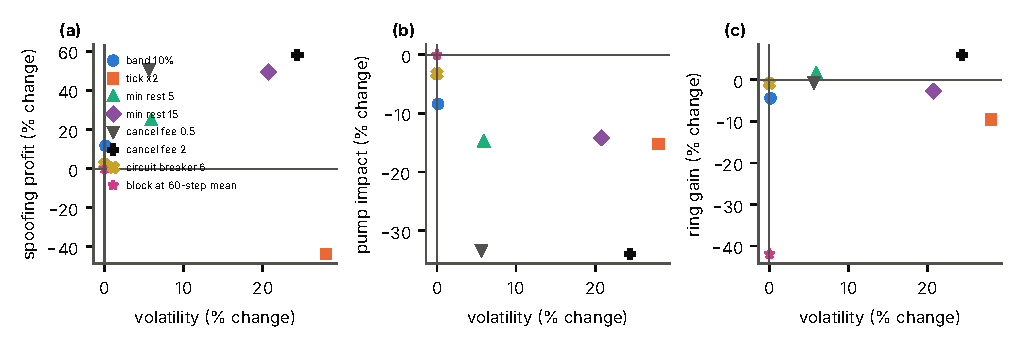
\includegraphics[width=\linewidth]{figures/tradeoff.pdf}
\caption{Effect on manipulators against cost to honest participants, first calibrated market. Each point is an order-level rule or band setting; the horizontal axis is the change of the honest-only volatility, the vertical axis the change in (a) spoofing profit, (b) pump impact and (c) ring gain, relative to the market with a 7\% band and no other rule. Manipulators do not adapt}\label{fig:tradeoff}
\end{figure}

\begin{table}[t]
\centering\scriptsize
\setlength{\tabcolsep}{3pt}
\adjustbox{max width=\linewidth}{\begin{tabular}{lrrrrrrrrr}
\toprule
policy & spread & depth & volatility & retail cost & volume & spoof impact & pump impact & wash share & ring gain \\
\midrule
band 7\% (today) & +0\% & +0\% & +0\% & +0\% & +0\% & 0.11 & 0.47 & 0.033 & 34k \\
band 10\% & -0\% & -0\% & +0\% & -2\% & -0\% & 0.14 & 0.43 & 0.033 & 32k \\
tick x2 & +35\% & -9\% & +28\% & -16\% & +7\% & 0.21 & 0.40 & 0.031 & 30k \\
min rest 5 & +2\% & -1\% & +6\% & -5\% & -0\% & 0.16 & 0.40 & 0.033 & 34k \\
min rest 15 & +7\% & -3\% & +21\% & -12\% & +1\% & 0.26 & 0.40 & 0.032 & 33k \\
cancel fee 0.5 & +2\% & -2\% & +6\% & -5\% & +1\% & 0.18 & 0.31 & 0.032 & 33k \\
cancel fee 2 & +8\% & -6\% & +24\% & -5\% & +5\% & 0.20 & 0.31 & 0.031 & 36k \\
circuit breaker 6 & -0\% & -0\% & -0\% & +1\% & -0\% & 0.15 & 0.45 & 0.033 & 33k \\
block at 60-step mean & +0\% & +0\% & +0\% & +0\% & +0\% & 0.11 & 0.47 & 0.033 & 20k \\
\bottomrule
\end{tabular}
}
\caption{First calibrated market, 10 honest-only and 24 manipulated episodes per policy. Spread, depth, volatility, retail trading cost and volume are relative to the band-7\% market; spoofing and pump impact are in ticks; ``wash share'' is the share of volume traded between colluding accounts; ring gain is in tick-lots. Manipulators do not adapt. Retail cost includes fees paid; it falls under larger ticks and fees because simulated noise traders mostly post passive orders and earn the spread.}\label{tab:matrix}
\end{table}

\subsection{Checking a lever against reality: the 2016 tick-size reform}\label{sec:tick}

The tick size is the one lever in the simulator for which a real natural experiment is available in public data. On 12 September 2016 the Ho Chi Minh Stock Exchange reduced its minimum tick (to 10, 50 and 100 VND below 10,000, between 10,000 and 49,950, and above 50,000 VND), while HNX and UPCoM stocks were not affected \citep[according to][]{vo2023}. Using daily open, high, low, close and volume, we compare 282 HOSE stocks with 489 control stocks over the 40 trading days before and the 40 days from one week after the reform. Outcomes are the Corwin--Schultz high-low spread estimator, the daily range, the absolute return, the share of zero-return days and log volume. We could not establish the old tick from our sources (one summary gave 500 VND for all prices, which cannot be right given the small observed spread change), so we compare with simulated reductions of the tick by factors of 2, 5 and 10.

Table~\ref{tab:tickcompare} and Figure~\ref{fig:tick} show the result. The share of zero-return days fell by 7.1 points relative to controls (95\% interval $-9.2$ to $-5.0$), by 8.3 points with 20-day windows and by 6.7 with 60-day windows, a larger change than in any of four placebo dates; the spread estimate fell by 0.06 points (8\% of its pre-reform level; interval $-0.13$ to $0.01$), and by 0.07 points with 60-day windows, with placebo estimates ranging from $-0.06$ to $+0.09$. By price tercile the fall in the spread estimate is concentrated in low-priced stocks ($-0.18$ points, interval $-0.32$ to $-0.03$, against a pre-reform level of 1.0\%). The simulator predicts a fall of the share of zero-return days by 38\% for a halving of the tick, 43\% for a five-fold cut and 78\% for a ten-fold cut (real: 24\%), and of the spread estimate by 21\%, 65\% and 85\% (real: 8\%). The signs agree, in line with the finding of lower trading costs by \citet{vo2023} on intraday data; the real effect is of the order of the simulator's prediction for a halving of the tick and much smaller than for a five- or ten-fold cut. Prices in the panel are adjusted, so price bands are approximate, and the design cannot separate the reform from other changes on HOSE in the same weeks.

\begin{figure}[t]
\centering
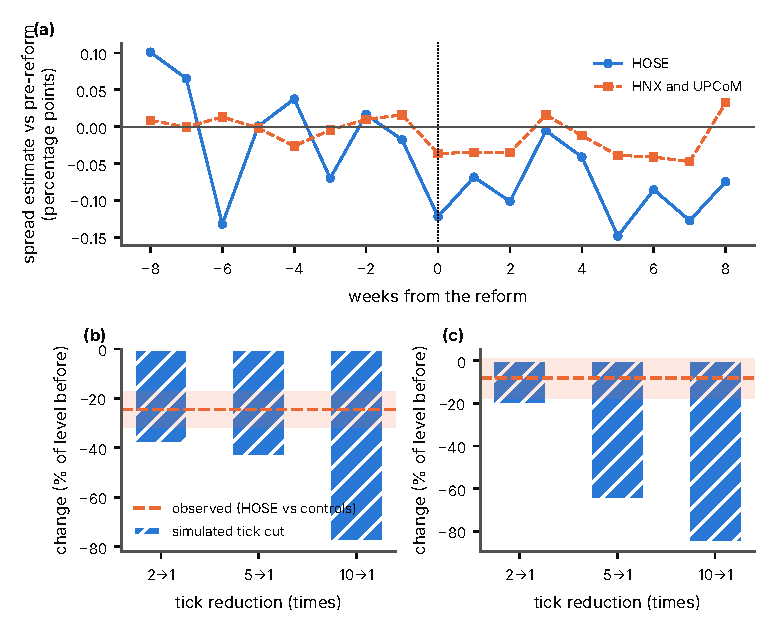
\includegraphics[width=\linewidth]{figures/tick.pdf}
\caption{The 2016 tick reform. (a) Weekly change of the Corwin--Schultz spread estimate relative to the 40 days before the reform for 282 HOSE stocks and 489 controls. (b), (c) Simulated change after a tick reduction by a factor of 2, 5 and 10 (bars) against the observed difference-in-differences (dashed line, shaded 95\% interval), as a percentage of the level before, for the share of zero-return days (b) and the spread estimate (c)}\label{fig:tick}
\end{figure}

\begin{table}[t]
\centering\scriptsize
\setlength{\tabcolsep}{3pt}
\adjustbox{max width=\linewidth}{\begin{tabular}{lccccc}
\toprule
outcome & real DiD (95\% interval) & real, relative to HOSE pre-period level & sim: tick $2\to1$ & $5\to1$ & $10\to1$ \\
\midrule
CS spread (\%) & -0.061 [-0.133, 0.008] & -8\% & -21\% & -65\% & -85\% \\
daily range (\%) & -0.067 [-0.213, 0.116] & -2\% & -7\% & -31\% & -50\% \\
|return| (\%) & -0.141 [-0.270, 0.012] & -8\% & -3\% & -35\% & -44\% \\
zero-return share & -0.071 [-0.092, -0.050] & -24\% & -38\% & -43\% & -78\% \\
log volume & -0.000 [-0.153, 0.172] & -- & -- & -- & -- \\
\bottomrule
\end{tabular}
}
\caption{Tick-size reform: real difference-in-differences against the simulator's prediction for a reduction of the tick by a factor of 2, 5 or 10. Changes relative to the pre-reform level.}\label{tab:tickcompare}
\end{table}

\subsection{Summary of the policy evidence}

Table~\ref{tab:summary} lists, for each lever, what the simulated markets and the real data show.

\begin{table}[t]
\centering\footnotesize
\begin{adjustbox}{max width=\linewidth}
\begin{tabular}{p{3.1cm}p{4.2cm}p{3.6cm}p{3.6cm}}
\toprule
lever & against rings & against spoofing, pumps, wash & cost to honest investors\\
\midrule
inspection with a fine proportional to the gain & deters with enough capacity (three accounts per window: 5 of 6 markets in each family); capacity falls by a factor of 2.4 when the fine multiple doubles & not tested & fine paid by manipulators only; inspection effort\\
off-book block priced at a trailing mean & removes 58--61\% of the block value at 60 steps and 87--98\% at one day; total gain falls to 28--44\% of its value at one day (block of 3000 lots; Appendix~\ref{app:extra}) & not applicable & 0.17\%--0.50\% of price on block trades\\
daily price band 7\% or 10\% & no effect in the markets tested & not tested & none observed in honest markets\\
minimum resting time, cancel fee & no effect & no reduction; spoofing profit and impact not lower & volatility +6\% to +24\%, spread up to +8\%\\
tick size & not tested for rings & larger tick lowers spoofing profit & spread +35\% for a doubled tick; real tick cut improved liquidity\\
\bottomrule
\end{tabular}
\end{adjustbox}
\caption{Policy evidence in this paper (simulated markets calibrated to Vietnam unless stated; the tick row also uses real data).}\label{tab:summary}
\end{table}


\section{Experiments III: real data}\label{sec:real}

\subsection{Real account-level order flow}\label{sec:real-accounts}

Every result above is for simulated accounts. To see what the statistic does on real accounts we use two public data sets from a venue with an account identifier on every record, the Hyperliquid derivatives exchange. They are far from the Vietnamese market (a crypto perpetual-futures venue, dominated by automated accounts, with pseudonymous addresses that one operator may use in several copies), so the results are a stress test of the statistic, not an estimate for Vietnam. There are no manipulation labels.

\paragraph{Data.} \emph{Order submissions}: the Level-4 order data of \citet{albers2026} (Zenodo record 18184441, CC BY 4.0), first member of the December 2025 file for the SOL perpetual, 577,918 orders submitted by 1,909 accounts in 23.6 minutes of 1 December 2025; we use one record per order identifier and the side of the order, windows of 300 bins of 0.5 seconds (150 seconds; nine windows with 351 to 715 active accounts and 61,000 orders on average). \emph{Fills}: a public table of fills (account address, side, millisecond time) of a 91-minute slice of 5 June 2026 for the perpetual contracts HYPE, BTC and ETH, windows of 300 bins of one second (18 windows). Accounts with fewer than three records in a window are not tested.

\paragraph{Calibration on real flow.} Table~\ref{tab:realcal} gives the share of accounts with small $p$-values. On submissions, 28.5\% of accounts with at least three orders in a window have $p\le0.01$ for the signed statistic (33.4\% unsigned), against a nominal 1\%, and the share rises with activity: 6.6\% for accounts with 3 to 9 orders, 32.6\% for 10 to 99, 51.8\% for 100 or more; for accounts that trade on both sides it is 43.6\%. Netting buys against sells barely lowers the rate, unlike in the simulator: real market makers do not re-quote symmetrically but shift both quotes in the direction of the last price move, so their net flows are positively correlated (Proposition~\ref{prop:netting} covers the symmetric case only). The exchangeability condition of Proposition~\ref{prop:exact} is violated for a large share of the active accounts of this venue: they react to the same signals. The aggregate flow of the other accounts is also dominated by a few loud accounts: its variance per bin, divided by the median variance of a quiet account (3 to 15 orders in the window), gives an effective number of accounts $N_{\mathrm{eff}}\approx10^6$ (Section~\ref{sec:power}) against about 470 accounts, so that a ring of quiet accounts is nearly invisible unless it is loud. On fills the pattern is mechanical and different: the signed statistic flags almost nothing (0.0--0.03\%) and the unsigned one 15--17\%, because each trade appears twice, as the buy of one account and the sell of its counterparty in the same millisecond, so that the aggregate of the others contains the mirror image of every account's own flow. The test must be applied to submissions, not to executed trades.

\begin{table}[t]
\centering\footnotesize
\adjustbox{max width=\linewidth}{\begin{tabular}{llrrrrr}
\toprule
data & accounts & account-windows & unsigned, $p\le0.01$ & signed, $p\le0.01$ & unsigned, $p\le0.05$ & signed, $p\le0.05$ \\
\midrule
fills, BTC & all with $\ge3$ & 3765 & 0.156 & 0.000 & 0.298 & 0.000 \\
fills, ETH & all with $\ge3$ & 1930 & 0.166 & 0.000 & 0.308 & 0.000 \\
fills, HYPE & all with $\ge3$ & 3732 & 0.151 & 0.000 & 0.290 & 0.001 \\
order submissions, SOL & 3--9 submissions & 843 & 0.075 & 0.066 & 0.198 & 0.206 \\
order submissions, SOL & 10--99 & 645 & 0.332 & 0.326 & 0.457 & 0.437 \\
order submissions, SOL & $\ge100$ & 682 & 0.655 & 0.518 & 0.723 & 0.594 \\
order submissions, SOL & all with $\ge3$ & 2170 & 0.334 & 0.285 & 0.440 & 0.397 \\
order submissions, SOL & both sides & 1166 & 0.525 & 0.436 & 0.624 & 0.534 \\
\bottomrule
\end{tabular}
}
\caption{Share of accounts flagged on real account-level flow (accounts with at least three records in the window). Under the null of Proposition~\ref{prop:exact} the share would be at most the level}\label{tab:realcal}
\end{table}

\paragraph{A ring planted in real flow.} To measure power against the real background, we choose $K=12$ quiet real accounts (3 to 15 orders in the window) and add to each, at ten common bins of the window (each member jittered by at most one bin), $q$ buy orders; the other accounts' flow is unchanged. Table~\ref{tab:realplant} and Figure~\ref{fig:realacc} give catch@$B$ over 180 trials (nine windows, 20 draws each). With no planting ($q=0$) none of the chosen accounts reaches the top five. A ring of three orders per push is undetectable; at 30 orders per member and push (5.9\% of the orders of the window in total) it is in the top ten in none of the 180 trials although 41\% of its members have $p\le0.01$, because more than a quarter of all accounts have $p\le0.01$ for natural reasons and the ranking is filled by loud accounts; at 100 orders (19.5\% of the flow of the window) it is in the top five in 80\% of the trials (signed statistic), and at 300 in all. The dependence on the design is steep and in the direction of Proposition~\ref{prop:power}: catch@5 falls from 1.00 to 0.79 as the number of accounts rises from 100 to 468 (by dropping real accounts at random), it is 0 for a ring of four, 0.26 for eight and 1.00 for 16 accounts, and 0.22, 0.79 and 1.00 for three, ten and thirty pushes per window. A ring of 12 retail accounts that submits a few orders at each of ten moments would not be found in this venue by this statistic; a ring that makes up a fifth of the flow of a stock-window would be. Whether a Vietnamese stock has a background as loud as this one is the empirical question account-level data would settle, and the planted-ring audit is the way to measure it (Section~\ref{sec:discussion}).

\begin{figure}[t]
\centering
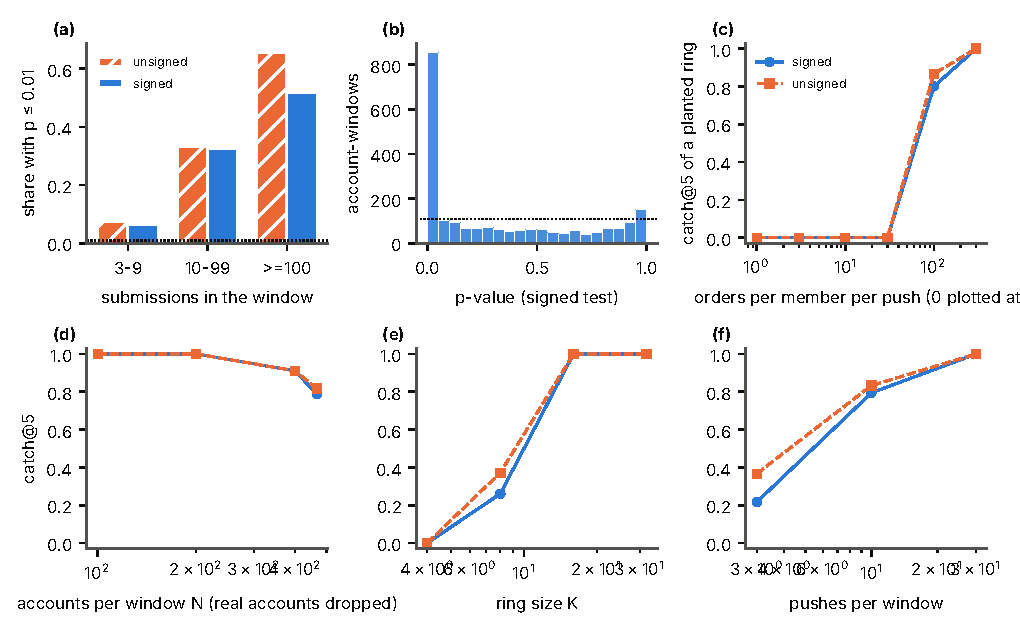
\includegraphics[width=\linewidth]{figures/real_accounts.pdf}
\caption{The coincidence test on real order submissions (SOL perpetual, 23.6 minutes). (a) Share of accounts with $p\le0.01$ by number of submissions in the window; dotted: nominal 1\%. (b) Histogram of signed-test $p$-values of accounts with at least three submissions; dotted: uniform. (c)--(f) catch@5 of a ring of 12 quiet real accounts planted at ten common moments per window, signed (solid) and unsigned (dashed), against the number of orders per member and push (c), the number of accounts (d), the ring size (e) and the number of pushes per window (f); unless varied, $q=100$ orders per push and the full set of accounts}\label{fig:realacc}
\end{figure}

\begin{table}[t]
\centering\scriptsize
\setlength{\tabcolsep}{3pt}
\adjustbox{max width=\linewidth}{\begin{tabular}{lrrrrrrrrr}
\toprule
sweep & $N$ & $K$ & orders per push & pushes & unsigned @5 & signed @1 & signed @5 & signed @10 & members with $p\le0.01$ \\
\midrule
orders per push & 468 & 12 & 0 & 10 & 0.00 & 0.00 & 0.00 & 0.00 & 0.09 \\
orders per push & 468 & 12 & 3 & 10 & 0.00 & 0.00 & 0.00 & 0.00 & 0.03 \\
orders per push & 468 & 12 & 10 & 10 & 0.00 & 0.00 & 0.00 & 0.00 & 0.06 \\
orders per push & 468 & 12 & 30 & 10 & 0.00 & 0.00 & 0.00 & 0.00 & 0.41 \\
orders per push & 468 & 12 & 100 & 10 & 0.87 & 0.59 & 0.80 & 0.89 & 1.00 \\
orders per push & 468 & 12 & 300 & 10 & 1.00 & 1.00 & 1.00 & 1.00 & 1.00 \\
accounts & 100 & 12 & 100 & 10 & 1.00 & 1.00 & 1.00 & 1.00 & 1.00 \\
accounts & 200 & 12 & 100 & 10 & 1.00 & 1.00 & 1.00 & 1.00 & 1.00 \\
accounts & 400 & 12 & 100 & 10 & 0.91 & 0.78 & 0.91 & 0.96 & 1.00 \\
accounts & 468 & 12 & 100 & 10 & 0.82 & 0.65 & 0.79 & 0.91 & 1.00 \\
ring size & 468 & 4 & 100 & 10 & 0.00 & 0.00 & 0.00 & 0.00 & 0.38 \\
ring size & 468 & 8 & 100 & 10 & 0.37 & 0.19 & 0.26 & 0.29 & 0.91 \\
ring size & 468 & 16 & 100 & 10 & 1.00 & 1.00 & 1.00 & 1.00 & 1.00 \\
ring size & 468 & 32 & 100 & 10 & 1.00 & 0.99 & 1.00 & 1.00 & 1.00 \\
pushes per window & 468 & 12 & 100 & 3 & 0.37 & 0.17 & 0.22 & 0.24 & 0.85 \\
pushes per window & 468 & 12 & 100 & 10 & 0.83 & 0.64 & 0.79 & 0.86 & 1.00 \\
pushes per window & 468 & 12 & 100 & 30 & 1.00 & 1.00 & 1.00 & 1.00 & 1.00 \\
\bottomrule
\end{tabular}
}
\caption{Planted ring among 12 quiet real accounts: catch@$B$ over 180 trials (nine windows, 20 draws), ranking by the signed statistic (unsigned at 5 for comparison), and share of members with $p\le0.01$. The sweep column names the factor that varies; the others are at $N=468$, $K=12$, 100 orders per push and 10 pushes}\label{tab:realplant}
\end{table}


\subsection{Documented enforcement cases on daily prices}\label{sec:cases}

\paragraph{Data and protocol.} Ten decisions of the State Securities Commission with exact dates of the conduct were collected from press reports quoting the decisions (Appendix~\ref{app:cases}; the decision documents were not opened). For every stock and date, using only data up to that date, we compute market-adjusted abnormal return, volume surge against the stock's own history, a round-trip statistic, the position of the close in the daily range, the count of days with moves of at least 6.5\%, and range expansion; stocks are ranked against each other on each date. The protocol, fixed before the cases were scored, is: a case stock is scored by the highest rank it reaches on any date in its period; two nulls are used, 300 random stocks over the same dates and 300 non-overlapping periods of the same length of the same stock; and we count the cases in which the stock is among the $B$ highest of its date at least once.

\paragraph{Results.} Table~\ref{tab:cases} gives the results. The market-adjusted abnormal return alone places 8 of the 10 cases in the daily top ten of about 1,360 scored stocks at some point of their period, against 15\% for random stocks over the same dates, and a case stock beats a random stock with probability 0.89 and the same stock at other times with probability 0.87. These are not stocks that rank high at all times. Combining six features, or an isolation forest on them, is no better than the single feature. Volume surge behaves differently in the two comparisons: against the same stock at other times it is informative (superiority 0.90, five of ten cases with $p<0.05$), against other stocks it is not (0.33), because other stocks have larger surges at some time; we therefore claim nothing new for the market-level detector. Table~\ref{tab:window} shows that the abnormal-return result is stable across window lengths of 10, 20 and 60 days (superiority over random stocks 0.87, 0.89, 0.85; over the same stock 0.78, 0.87, 0.89). The result says little about precision: periods are long (83 to 587 trading days), only ten cases are documented among thousands of price run-ups, and an unlabelled run-up is not an innocent one.

\begin{table}[t]
\centering\footnotesize
\adjustbox{max width=\linewidth}{\begin{tabular}{lrrrrrrr}
\toprule
detector & superiority & top 10 & chance & top 20 & chance & top 50 & chance \\
\midrule
market-adjusted abnormal return & 0.89 & 8/10 & 15\% & 10/10 & 27\% & 10/10 & 53\% \\
combined six-feature score & 0.78 & 6/10 & 22\% & 6/10 & 35\% & 10/10 & 58\% \\
isolation forest, same features & 0.78 & 7/10 & 21\% & 8/10 & 34\% & 9/10 & 54\% \\
round trip (run-up, retracement) & 0.70 & 9/10 & 76\% & 10/10 & 81\% & 10/10 & 90\% \\
volume surge & 0.33 & 0/10 & 3\% & 0/10 & 5\% & 0/10 & 13\% \\
\bottomrule
\end{tabular}
}
\caption{Ten documented cases scored against about 1,360 stocks (20-day window). Superiority is the probability that a case stock beats a random stock (0.5 is chance); ``top $B$'' counts cases in which the stock reached the daily top-$B$ list at some date of its period; ``chance'' is the same share for random stocks.}\label{tab:cases}
\end{table}

\begin{table}[t]
\centering\footnotesize
\adjustbox{max width=\linewidth}{\begin{tabular}{llrrr}
\toprule
window (days) & detector & superiority vs random stocks & superiority vs same stock & cases in top 10 / 10 \\
\midrule
10 & abnormal return & 0.87 & 0.78 & 9 \\
10 & combined score & 0.69 & 0.70 & 5 \\
10 & volume surge & 0.33 & 0.88 & 0 \\
20 & abnormal return & 0.89 & 0.87 & 8 \\
20 & combined score & 0.79 & 0.86 & 6 \\
20 & volume surge & 0.33 & 0.90 & 0 \\
60 & abnormal return & 0.85 & 0.89 & 3 \\
60 & combined score & 0.77 & 0.88 & 3 \\
60 & volume surge & 0.28 & 0.79 & 0 \\
\bottomrule
\end{tabular}
}
\caption{Sensitivity to the window length. Superiority against random stocks and against the same stock at other times; number of cases in the daily top ten.}\label{tab:window}
\end{table}

\paragraph{Event time.} Figure~\ref{fig:cases} aligns the ten cases at the first day of their documented period. The cumulative market-adjusted return of the case stocks is flat before the period and rises through it (mean $+0.29$ twenty days after the start and $+0.42$ after sixty), the mean percentile of the abnormal-return score rises from 0.39 sixty days before to 0.78 twenty days after, and the percentile of the volume-surge score does not rise consistently (0.34 at day $-60$, 0.41 at day 20, 0.28 at day 60), which is the reading of Table~\ref{tab:cases} in time: the price runs up on ordinary volume.

\begin{figure}[t]
\centering
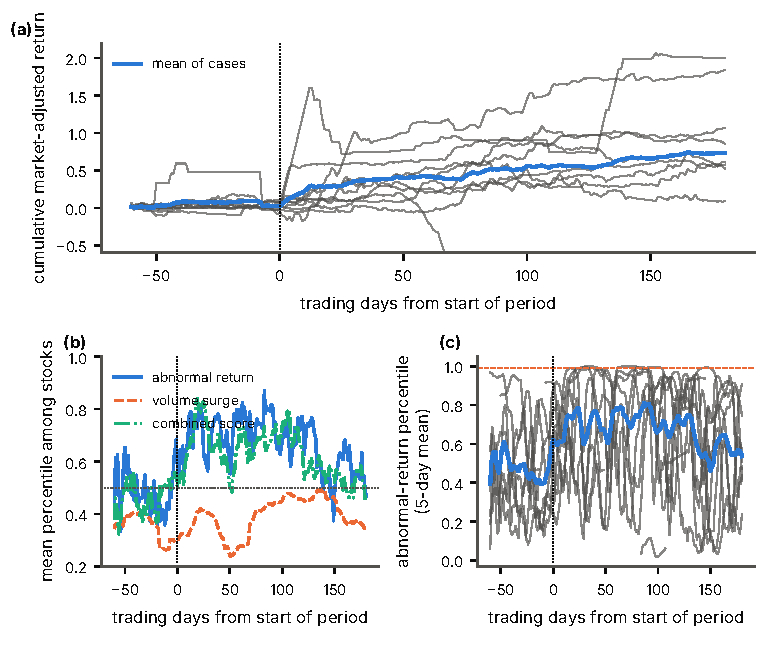
\includegraphics[width=\linewidth]{figures/cases.pdf}
\caption{The ten documented cases in event time (day 0 is the first day of the documented period). (a) Cumulative market-adjusted log return since day $-60$: individual cases (grey) and mean (blue). (b) Mean cross-sectional percentile among all stocks of three scores computed from data up to each day (20-day windows). (c) Percentile of the abnormal-return score, 5-day moving average, individual cases (grey) and mean (blue); dashed line: the 99th percentile}\label{fig:cases}
\end{figure}

\paragraph{Case stocks and the daily band.} Table~\ref{tab:casestats} compares the case stocks with the market and counts days within 0.5 points of the daily ceiling. The stocks are ordinary (median daily volatility 1.75\% in the year before against 2.46\% for HOSE stocks), and the band is reached in their manipulation periods: five ceiling days at the median, and runs of up to 12 days. This differs from the simulated ring, whose price displacement of about 0.5\% never reaches the band. The band could matter for a manipulator who ratchets the price over days; our simulated rings do not, so the finding that the band has no effect is a statement about rings of the size we simulate, not about all manipulation.

\begin{table}[t]
\centering\footnotesize
\adjustbox{max width=\linewidth}{\begin{tabular}{llrrrrrrr}
\toprule
stock & exchange & days & pre-period vol. (\%) & vol. in period (\%) & zero-return share & log price change ($\times100$) & ceiling days & longest run \\
\midrule
FIR & HOSE & 109 & 1.63 & 1.84 & 0.02 & +38 & 0 & 0 \\
SJS & HOSE & 192 & 2.32 & 2.34 & 0.13 & +49 & 10 & 3 \\
PDR & HOSE & 83 & 1.94 & 3.84 & 0.07 & -119 & 4 & 3 \\
PSH & unknown & 319 & 1.75 & 3.45 & 0.45 & -12 & 26 & 3 \\
AGG & HOSE & 514 & 1.29 & 1.90 & 0.13 & +35 & 7 & 1 \\
CRC & HOSE & 106 & 1.36 & 2.65 & 0.18 & +73 & 5 & 1 \\
GKM & HNX & 125 & 1.62 & 3.77 & 0.32 & +157 & 1 & 1 \\
PAS & UPCOM & 491 & 3.37 & 3.54 & 0.10 & -87 & 0 & 0 \\
HCI & unknown & 146 & 6.78 & 6.17 & 0.81 & +183 & 21 & 12 \\
\bottomrule
\end{tabular}
}
\caption{Case stocks: daily volatility and zero-return share in the year before the period, volatility during it, price change over the period, days within 0.5 points of the daily ceiling and the longest run of such days.}\label{tab:casestats}
\end{table}

\subsection{Telegram-organised pump events on tick data}\label{sec:pump}

We use a public archive of 701 pump events with trades from about 24 hours before the pump time to shortly after (Appendix~\ref{app:calib}). The files hold side, price and amount, with no account identifiers, so the coincidence test cannot be applied. For each event, standardised volume and buy imbalance over rolling ten-minute windows are measured against the same coin's first 20 hours. Figure~\ref{fig:pump} shows accumulation: mean standardised volume rises from 0.19 (4 to 3 hours before) to 0.71 (last ten minutes), and buy imbalance from 0.03 to 0.23, with intervals excluding zero, and both jump at the pump. This supports the accumulate--push structure of the simulated ring. It does not give early warning: with the alarm rate in the background set to 0.05 per coin-hour, only 6.0\% of events raise an alarm in the last hour before the pump (8.3\% at 0.1 and 16.4\% at 0.25 per coin-hour; median lead 7 to 15 minutes when it fires).

\begin{figure}[t]
\centering
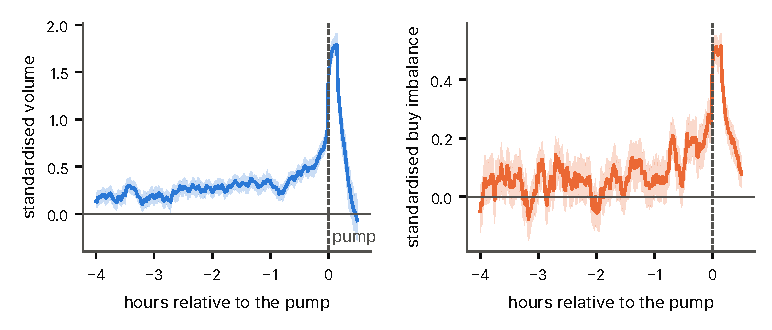
\includegraphics[width=0.85\linewidth]{figures/pump.pdf}
\caption{Standardised volume and buy imbalance of 701 pump events around the pump time (mean and 95\% bootstrap interval over events)}\label{fig:pump}
\end{figure}




\section{Discussion: what this means for a regulator}\label{sec:discussion}

The evidence is simulated for the questions on rules and real for some of the questions on data, and the two do not overlap on accounts. We therefore separate what a regulator could act on now, what it should do to learn more before acting, and what should not be concluded.

\subsection{Findings that can guide rules now}

\paragraph{Price off-book blocks from a trailing mean.} Among the price and order rules we tested this is the only one that cuts the ring's gain through a mechanism that can be written down and checked: a reference price that averages the last $L$ prices credits a push only for increments that are recent and discounts them linearly with age (Proposition~\ref{prop:block}). In the simulated markets a one-day reference removes 87\% (index level) to 98\% (stock level) of the value of the block and leaves the ring between a tenth and a half of its total gain (Section~\ref{sec:blockcheck}); this holds for a block of the assumed size, and a ring whose gain is mostly trading profit (blocks ten times smaller) keeps more than 80\% of it; a ring can recover the value only by holding the price for about $L-a/2$ steps, which is itself the conduct to deter. Its cost to honest trading is the gap between the last price and the trailing mean on block trades, 0.2\% to 0.5\% of the price in our first preset, which we have not measured on real negotiated trades. One of the ten documented cases (PSH) was carried out on a negotiated system, and the rule applies where the ring's gain is realised off the order book; it does nothing against manipulation that profits on the book. We would pilot it first on a small set of stocks and compare negotiated-trade prices with the trailing mean to measure the cost before it binds.

\paragraph{Inspection capacity and the fine are exchangeable.} With a fine proportional to the gain, deterrence requires only that the probability of being caught exceed $1/m$ (Proposition~\ref{prop:deter}). Under the fitted power law, doubling the fine multiple from five to ten cuts the capacity needed to deter a small ring by a factor of about 2.4 (3.0 to 1.2 inspected accounts per window at 600 active accounts; Table~\ref{tab:capacity}). The Vietnamese caps (five times the gain for individuals, ten for organisations, as reported by the press) therefore matter for how many accounts the inspectorate must examine, and an increase in the cap for individuals would be worth about as much as a 2.4-fold increase in capacity under our model. The empirical counterpart is the finding of \citet{comerton2014} that the regulator's budget has a strong effect on both manipulation and detection. The arithmetic of a workload is simple: $B$ inspected accounts per window, $S$ stocks and $W$ windows per year give $BSW$ account reviews a year; with $B=3$, an illustrative 400 stocks and about 200 windows (a window is about 300 minutes), that is 240,000 automated reviews a year, of which only the highest-ranked need human attention. Because the saving from screening shrinks as the number of accounts per stock grows (Table~\ref{tab:capacity}: saving of 3.7 at 600 accounts and 2.0 at 2000), capacity should be allocated first to stocks with few active accounts, where screening is most informative.

\paragraph{Do not use order-level frictions or the band against rings.} Minimum resting times and cancel fees did not reduce spoofing, pump-and-dump or wash trading in the calibrated market and cost honest participants 7--8\% in spread and 21--24\% in volatility at the strictest settings; a larger tick widened the spread by 35\% (Figure~\ref{fig:tradeoff}). Widening the daily band to 10\% or 15\% changed nothing for rings of the simulated size. These results are conditional on the simulator: the ring moves the price by about 0.5\% and never reaches the band, whereas the case stocks reached the ceiling for a median of five days and, for one stock, 12 in a row (the band of that stock is assumed) (Table~\ref{tab:casestats}). Whether the band constrains a ring that ratchets the price over days is a question for account-level data.

\paragraph{Do not undo the 2016 tick reform.} On the data we have, the reduction of the tick on HOSE in 2016 lowered the share of zero-return days by 7.1 points relative to control exchanges, a larger change than at four placebo dates, and the estimated spread by about 8\% (the interval includes zero), in the direction the simulator predicts and consistent with lower trading costs found on intraday data \citep{vo2023}. Tick size is a liquidity instrument and is not a manipulation instrument: we found no evidence that it deters rings, and the doubling of the tick in the simulator costs honest participants a third of the spread.

Table~\ref{tab:options} puts the options side by side with the strength of the evidence behind each and the first step a regulator could take.

\begin{table}[t]
\centering\footnotesize
\begin{adjustbox}{max width=\linewidth}
\begin{tabular}{p{2.7cm}p{3.3cm}p{2.5cm}p{3.0cm}p{2.9cm}}
\toprule
option & effect found & evidence & cost or risk & first step\\
\midrule
price off-book blocks from a trailing mean ($L\approx$ one day) & removes 87--98\% of the block value; total ring gain falls to 28--44\% (for the assumed block of 3000 lots) & simulated, two families, with an exact ex-post check and a closed-form law & 0.2--0.5\% gap to the last price on block trades (not measured on real trades) & compare negotiated-trade prices with trailing means on a few stocks\\
higher fine multiple, or more inspection capacity & doubling the multiple from 5 to 10 cuts the capacity needed to deter by a factor of 2.4 & simulated; closed form fitted to the agent-based market at about 100 accounts and extrapolated with $N^{-1/2}$; weaker in markets with more accounts (2 of 4 without trending) & legal change; staff; false flags & compute the workload $BSW$; plan capacity by number of accounts per stock\\
screening in shadow mode on account-level data & measures the share of accounts flagged and the effective number of accounts & real order flow elsewhere shows the null fails; none for Vietnam & data governance; interpretation of flags & planted-ring audit on the regulator's own history\\
no minimum resting time, cancel fee or larger tick as anti-manipulation tools & avoids +7--8\% spread, +21--24\% volatility, +35\% spread & simulated; tick reform on real data & none & none\\
change of the daily band & none for rings of the simulated size & simulated; case stocks reach the ceiling & unknown for rings that ratchet the price & study case stocks with account data\\
\bottomrule
\end{tabular}
\end{adjustbox}
\caption{Options for the regulator, the effect found, the strength of the evidence, cost or risk, and a first step.}\label{tab:options}
\end{table}

\subsection{What a regulator should do to learn more before relying on the test}

\paragraph{Run the test in shadow mode on account-level data.} The one thing that would change our conclusions most is access to account-level order data, which only the exchange, the depository and the commission hold. On such data the first deliverable is not a ranking of accounts but the calibration check of Section~\ref{sec:real-accounts}: the share of accounts with small $p$-values by activity tier, which measures how far the exchangeability condition is violated in that market.

\paragraph{Audit the detector with planted rings in the regulator's own history.} The planted-ring experiment on real order flow (Section~\ref{sec:real-accounts}) is a procedure that does not need labels: inject synthetic coordinated orders into a historical window, vary the size, activity and number of accounts, and measure catch@$B$ against the real background of the stock in question. It yields the capacity $B$ needed per stock for a target detection probability and reveals stocks in which the background of automated accounts makes the test uninformative. Because it uses the venue's own flow, it also estimates $s_0$ of~\eqref{eq:fit} for that venue.

\paragraph{Treat a flag as a screening signal, not as evidence.} The test controls false alarms per account only under an exchangeability condition that real order flow violates (Section~\ref{sec:real-accounts}); with ranking the guarantee is lost (Proposition~\ref{prop:budget}); and in an algorithm-dominated venue the highest-ranked accounts are likely to be honest bots that react to the same signals. The ranking is therefore an input to human review, with a documented route to appeal, not a basis for sanctions. In the simulator an honest fund that splits orders over sub-accounts is flagged at six times the nominal rate, and a regulator that acts on flags must expect to meet such cases.

\subsection{Risks and unintended effects}

\paragraph{Who bears the cost.} The block-price rule falls on those who trade off the order book; in the simulator it has no effect on honest trading because honest agents do not trade blocks, and its cost on real negotiated trades is not measured. Order-level frictions raise volatility and spreads for all participants (Table~\ref{tab:matrix}); the simulated retail trading cost falls under larger ticks and fees because simulated noise traders mostly post passive orders, which we regard as an artefact, so we do not rank who pays most. The fine falls on manipulators. Inspection has a burden of its own: with $B=3$ inspected accounts in each of 600 active accounts per window and 200 windows a year, an account chosen at random would be inspected $3\cdot200/600=1$ time a year, so that every honest account faces about one inspection a year if the ranking were uninformative, and in practice more for loud and automated accounts, which the ranking favours (Section~\ref{sec:real-accounts}). The burden is small in effort and potentially large in reputation, which is a reason to keep the first inspection a data request and not a sanction.

\paragraph{Displacement.} Under inspection the best-responding ring does not stop; it shrinks, to about 3\% of its unconstrained gain in the stock-level family. Deterrence of large rings may push manipulation toward smaller operations that fall below the inspection threshold, which is the right objective if harm is proportional to size and the wrong one if many small rings together do equal harm. The law of Proposition~\ref{prop:power} says where the threshold lies: a ring of $k$ co-active accounts is detectable if $k-1\gtrsim c\sqrt N$, so the threshold rises with the square root of the number of accounts.

\paragraph{Evasion once the rule is known.} A published rule invites a response. Our strategy space includes jitter (spreading members' actions in time) and cross trades, but the ring cannot, for example, trade across several stocks, split its activity over several windows with a different group of accounts, or imitate the order flow of an honest group. Randomising the inspected set among the top-ranked accounts, and keeping the exact statistic confidential, are measures we have not tested.

\paragraph{Privacy and governance.} Account-level surveillance data are sensitive. A shadow-mode pilot should run inside the exchange or the commission, with the output reduced to ranked pseudonymous identifiers, and with the false-flag statistics of the pilot published before any use for enforcement.

\subsection{Generalisation}

The structure that drives the results is not specific to Vietnam: a market dominated by retail investors, a daily price band, off-book or negotiated trades priced from a reference, administrative fines that are a multiple of the gain, and a regulator with limited inspection capacity. For another market, the quantities to re-estimate are the cancel share, the retail share, the volatility of the index and of a typical stock, the number of active accounts per stock, and the reference-price rule for blocks; the family-of-markets design then gives the distribution of the ring's value over markets that match those moments. The introduction of a new trading system in Vietnam in May 2025 may raise the share of automated accounts; Section~\ref{sec:real-accounts} shows that on a venue dominated by automated accounts the coincidence test flags many accounts and loses power, which is a reason to calibrate it on the new flow before relying on it; we did not vary the share of automated accounts.

\subsection{Limitations}

No real account-level data from Vietnam have been used, so we do not know whether real rings are separable from honest coordination by this test. The simulator's manipulators and honest groups were written by the same author as the detectors, and a model trained with labels in the simulator beats the label-free test in every scenario. The calibrated markets do not reproduce the spread, the tails or the absence of serial correlation in daily returns (Figure~\ref{fig:calibration}; a third family that restores it is analysed in Section~\ref{sec:acf}). Rule facts come from broker summaries and press, and we could not establish the pre-reform tick. The ring search has a small budget and the strategy set was found in the first market; the strategies were not re-optimised in each market of the families, so the reported effects of the rules are lower bounds on what an adaptive ring gains (Proposition~\ref{prop:lower}). The block value of 3000 lots is an assumption; a ring that is caught is assumed to be exposed by one inspected member; and fixed manipulators other than the ring are not best responses. The power law is an approximation fitted to 11 points with two constants. The real account-level data are pseudonymous addresses on a crypto derivatives venue, and the planted ring is synthetic. The Vietnamese checks are at the level of the stock; the case periods come from press reports; the panel holds only stocks that are still listed; the natural experiment compares HOSE with other exchanges in the same weeks and cannot rule out other differences.

\subsection{Next steps}

Account-level data from the exchange, or the per-account trade tables in published case files, would allow a direct test of the central claim. A rule based on finer resampling and a false-discovery-rate bound should replace top-$B$ ranking, whose sensitivity falls with the number of accounts. A test conditioned on the common drivers of order flow (price moves, news, activity regimes) is needed for algorithm-dominated markets. The interplay of an adaptive ring with an adaptive regulator is a repeated game that double-oracle methods could solve \citep{mcmahan2003,lanctot2017}. And the optimal combination of fine, capacity and rules is a design problem that the closed forms of Section~\ref{sec:deter} make tractable.

\section{Conclusion}

A regulator without labelled cases can screen for coordinated accounts with a test whose false-alarm rate is exact per account under an exchangeability condition, whose power falls like the inverse square root of the number of accounts, and whose failure profile we have measured on simulated honest groups and on real order flow. Against a ring that adapts, pricing off-book blocks at a trailing mean and a sufficient inspection capacity under a fine proportional to the gain remove most of the ring's expected benefit in simulated markets that match the observable moments of the Ho Chi Minh Stock Exchange (for the block rule, when the block is the main source of the ring's gain), while the daily band does not, and minimum resting times and cancel fees, tested in one market against fixed manipulators, do not and cost honest investors liquidity. The central uncertainty is the one data would settle: whether real rings in a retail-dominated market look like the simulated ones against a background of honest accounts that is as synchronised as the real one.


\backmatter

\begin{appendices}
\makeatletter\@removefromreset{table}{section}\@removefromreset{figure}{section}\makeatother
\renewcommand{\thetable}{\arabic{table}}\renewcommand{\thefigure}{\arabic{figure}}
\section{Documented cases used in Section~\ref{sec:real}}\label{app:cases}
\begin{table}[h]
\centering\footnotesize
\adjustbox{max width=\linewidth}{\begin{tabular}{llrll}
\toprule
ticker & period & accounts & decided & type \\
\midrule
FIR & 2022-01-04 to 2022-06-17 & 76 & SSC 2023-11 and 2024-01 & cross trading among own accounts \\
SJS & 2023-04-10 to 2024-01-10 & 26 & SSC 2026-01-08 & continuous buying and selling \\
PDR & 2022-08-15 to 2022-12-09 & 164 & SSC 2025-03-21 & cross trading among own accounts \\
PSH & 2021-02-01 to 2022-05-27 & 26 & SSC 2024-05-27 & negotiated trades within a group \\
AGG & 2020-12-01 to 2022-12-31 & 92 & SSC 2025-09 (year inferred) & continuous buying and selling \\
PPT & 2022-06-17 to 2024-10-17 & 19 & SSC decision 881 & continuous buying and selling \\
CRC & 2025-03-03 to 2025-08-01 & 10 & SSC 2025-12-22 & cross trading \\
GKM & 2021-08-02 to 2022-01-28 & 23 & SSC 2023-12-21 & fake supply and demand to push the price up \\
PAS & 2021-01-04 to 2022-12-30 & 19 & SSC 2026-02-12 & continuous buying and selling \\
HCI & 2019-12-13 to 2020-07-16 & 5 & SSC 2024-05-30 & cross matched orders among own accounts \\
HNG & 2015-07-20 to 2016-04-01 & 42 & SSC 2017-08-10 & multi-account fake supply and demand \\
\bottomrule
\end{tabular}
}
\caption{Cases with exact dates of the conduct. The periods are from press reports quoting the State Securities Commission decisions (sources are listed in the repository file \texttt{data/cases.csv}); the decision documents were not opened. FIR was the subject of two decisions with the same period and is counted once. PSH was traded on the negotiated system.}
\end{table}

\section{Sources for the calibration and real-data checks}\label{app:calib}
\begin{itemize}\itemsep0pt
\item Tick sizes, daily bands, lot sizes, sessions: broker rule summaries (FPTS for HOSE, a securities-company PDF for HNX); the system of the Korea Exchange (KRX) went live on 5 May 2025. Details and confidence tags: \texttt{docs/vietnam\_calibration.md} in the repository.
\item Fine cap of five times (individuals) and ten times (organisations) the illegal gain: Vietnamese press and legal-news summaries of Decree 156/2020 as amended; not read from the decree.
\item Cancel and amendment share of 31.76\% of orders (December 2020): press report of a HOSE statement.
\item VN30, VN-Index and VN100 bars and the VN30F1M ticks: public Kaggle datasets (keithvo/vnstockdata, khimduong/vn30-market-making).
\item Daily prices of 1,551 stocks: public Kaggle dataset (vuthinh/vietnam-stock-market-ohlc-price-data).
\item Pump events: public Hugging Face dataset (Go3x3/pump\_and\_dump\_dataset, MIT licence).
\item Order submissions with account identifiers: \citet{albers2026} (Zenodo record 18184441, CC BY 4.0), first member of the December 2025 SOL file of 877 million records per day over BTC, ETH and SOL; fills with account addresses: a public Hugging Face table of Hyperliquid fills (craftify2221/hyperliquid-fills-raw; the dataset card declares no licence), one row group of 5 June 2026. Both are mirrors or derivatives of the venue's public node data; we use samples of the files, not the full archives.
\item Exchange metadata (HOSE, HNX or UPCoM for each ticker): public Hugging Face table of Vietnamese stock symbols (kjhq/Vietnam-Stock-Symbols-and-Metadata).
\end{itemize}

\section{Single-market results}\label{app:single}
The first version of the policy comparison used one calibrated market (index level, daily volatility 1.14\%), with 20 selection and 20 reporting episodes per cell and seven strategies. Table~\ref{tab:policy} and Figure~\ref{fig:policy} are from it; they include the daily bands of 10\% and 15\% and a fine multiple of 10, and they are consistent with the family results (band: no effect; block price: large reduction; inspection: negative net benefit at one and three inspected accounts in that market).

\begin{figure}[h]
\centering
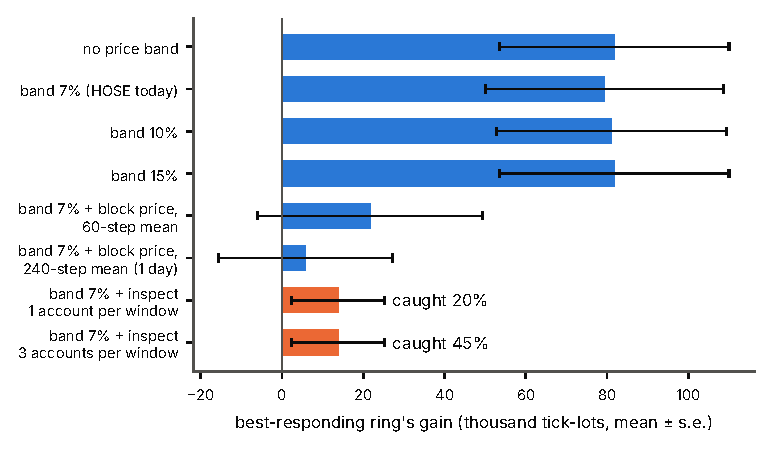
\includegraphics[width=0.85\linewidth]{figures/policy.pdf}
\caption{Single market: gain of the best-responding ring (thousand tick-lots, mean and standard error over 20 episodes)}\label{fig:policy}
\end{figure}

\begin{table}[h]
\centering\footnotesize
\adjustbox{max width=\linewidth}{\begin{tabular}{lrrrr}
\toprule
policy & ring gain (mean, s.e.) & caught & net benefit after fine, $m=5$ & $m=10$ \\
\midrule
no price band & 81.7k (28.3k) & -- & -- & -- \\
band 7\% (HOSE today) & 79.4k (29.3k) & -- & -- & -- \\
band 10\% & 81.1k (28.2k) & -- & -- & -- \\
band 15\% & 81.7k (28.3k) & -- & -- & -- \\
band 7\% + block at 60-step mean & 21.7k (27.6k) & -- & -- & -- \\
band 7\% + block at 240-step mean & 5.8k (21.4k) & -- & -- & -- \\
band 7\% + inspect 1 per window & 13.8k (11.4k) & 20\% & -35.6k & -85.1k \\
band 7\% + inspect 3 per window & 13.8k (11.4k) & 45\% & -48.9k & -111.6k \\
\bottomrule
\end{tabular}
}
\caption{Single market: best-responding ring against each policy; net benefit with fines of $m=5$ and $m=10$ times the gain.}\label{tab:policy}
\end{table}

\section{Additional tables}\label{app:extra}

Table~\ref{tab:calibmarkets} gives the moments of each accepted market re-measured over 16 honest episodes, and Table~\ref{tab:blocksize} the block-price rule against the assumed block size. Table~\ref{tab:ablation} gives the ablations of the signed test behind Figure~\ref{fig:sens}, and Table~\ref{tab:order} the effect of order-level rules on the default, non-adaptive spoofer in the uncalibrated simulator, which the main text does not use.

\begin{table}[h]
\centering\footnotesize
\adjustbox{max width=\linewidth}{\begin{tabular}{llrrrrr}
\toprule
family & market (draw) & volatility at acceptance (\%) & volatility, 16 episodes (\%) & cancel share & retail share & spread (ticks) \\
\midrule
index level & 1 & 1.08 & 1.10 (0.06) & 0.316 & 0.711 & 3.04 \\
index level & 5 & 1.13 & 1.63 (0.12) & 0.262 & 0.730 & 3.38 \\
index level & 11 & 1.08 & 1.26 (0.10) & 0.331 & 0.699 & 3.07 \\
index level & 19 & 1.17 & 1.40 (0.10) & 0.328 & 0.670 & 2.86 \\
index level & 20 & 0.93 & 1.19 (0.06) & 0.271 & 0.752 & 3.46 \\
index level & 26 & 1.18 & 1.22 (0.10) & 0.303 & 0.724 & 3.27 \\
stock level & 14 & 2.03 & 1.65 (0.08) & 0.277 & 0.728 & 3.45 \\
stock level & 19 & 2.19 & 2.58 (0.17) & 0.276 & 0.663 & 3.17 \\
stock level & 23 & 2.48 & 2.06 (0.14) & 0.302 & 0.692 & 3.35 \\
stock level & 39 & 2.19 & 2.23 (0.16) & 0.277 & 0.672 & 3.23 \\
stock level & 49 & 2.42 & 2.87 (0.23) & 0.265 & 0.695 & 3.43 \\
stock level & 61 & 1.84 & 1.81 (0.16) & 0.282 & 0.709 & 3.28 \\
\bottomrule
\end{tabular}
}
\caption{Moments of the accepted markets re-measured over 16 honest episodes of 6000 steps (standard error of the volatility in brackets), against the volatility measured at acceptance on two episodes. Tolerances: volatility 0.9--1.4\% (index level) and 1.8--2.8\% (stock level), cancel share 0.27--0.37, retail share 0.66--0.85}\label{tab:calibmarkets}
\end{table}

\begin{table}[h]
\centering\footnotesize
\adjustbox{max width=\linewidth}{\begin{tabular}{lrrrrrr}
\toprule
& \multicolumn{3}{c}{index level} & \multicolumn{3}{c}{stock level} \\
\cmidrule(lr){2-4}\cmidrule(lr){5-7}
block size (lots) & gain, last price & kept at $L=60$ & kept at $L=240$ & gain, last price & kept at $L=60$ & kept at $L=240$ \\
\midrule
300 & 42k & 0.89 & 0.83 & 68k & 0.92 & 0.87 \\
1000 & 70k & 0.74 & 0.60 & 101k & 0.78 & 0.64 \\
3000 & 151k & 0.52 & 0.28 & 297k & 0.68 & 0.44 \\
10000 & 435k & 0.49 & 0.19 & 693k & 0.53 & 0.21 \\
\bottomrule
\end{tabular}
}
\caption{Block-price rule against the assumed block size (median over six markets per family): gain with the last price as reference, and the share of it kept when the block is priced at the mean of the last 60 or 240 steps, for a ring that keeps its strategy. Assumed size: 3000 lots}\label{tab:blocksize}
\end{table}

\begin{table}[h]
\centering\footnotesize
\adjustbox{max width=\linewidth}{\begin{tabular}{llcccr}
\toprule
factor & level & catch@5 & catch@1 & honest flagged & accounts per window \\
\midrule
tolerances & (1,) & 0.89\,{\scriptsize[0.85, 0.94]} & 0.44\,{\scriptsize[0.38, 0.52]} & 0.013 & 100 \\
 & (1, 5) & 0.88\,{\scriptsize[0.83, 0.93]} & 0.55\,{\scriptsize[0.48, 0.62]} & 0.013 & 100 \\
 & (1, 5, 15) & 0.91\,{\scriptsize[0.86, 0.96]} & 0.56\,{\scriptsize[0.50, 0.63]} & 0.014 & 100 \\
 & (1, 5, 15, 30) & 0.90\,{\scriptsize[0.86, 0.95]} & 0.55\,{\scriptsize[0.49, 0.61]} & 0.014 & 100 \\
window length (steps) & 150 & 0.88\,{\scriptsize[0.83, 0.91]} & 0.41\,{\scriptsize[0.34, 0.47]} & 0.007 & 81 \\
 & 300 & 0.91\,{\scriptsize[0.86, 0.96]} & 0.56\,{\scriptsize[0.50, 0.63]} & 0.014 & 100 \\
 & 600 & 0.91\,{\scriptsize[0.84, 0.97]} & 0.58\,{\scriptsize[0.46, 0.71]} & 0.018 & 108 \\
noise traders (accounts) & 80 & 0.91\,{\scriptsize[0.86, 0.96]} & 0.56\,{\scriptsize[0.50, 0.63]} & 0.014 & 100 \\
 & 200 & 0.84\,{\scriptsize[0.76, 0.90]} & 0.45\,{\scriptsize[0.34, 0.55]} & 0.010 & 206 \\
 & 400 & 0.64\,{\scriptsize[0.55, 0.71]} & 0.17\,{\scriptsize[0.10, 0.25]} & 0.009 & 373 \\
 & 800 & 0.28\,{\scriptsize[0.24, 0.34]} & 0.08\,{\scriptsize[0.03, 0.14]} & 0.010 & 708 \\
ring size K & 4 & 0.79\,{\scriptsize[0.72, 0.85]} & 0.41\,{\scriptsize[0.33, 0.49]} & 0.013 & 93 \\
 & 8 & 0.88\,{\scriptsize[0.84, 0.94]} & 0.50\,{\scriptsize[0.42, 0.60]} & 0.012 & 97 \\
 & 16 & 0.94\,{\scriptsize[0.89, 0.97]} & 0.53\,{\scriptsize[0.44, 0.60]} & 0.012 & 104 \\
 & 30 & 0.94\,{\scriptsize[0.91, 0.97]} & 0.63\,{\scriptsize[0.56, 0.69]} & 0.012 & 115 \\
ring push probability & 0.2 & 0.46\,{\scriptsize[0.37, 0.55]} & 0.13\,{\scriptsize[0.08, 0.20]} & 0.012 & 100 \\
 & 0.4 & 0.79\,{\scriptsize[0.73, 0.87]} & 0.31\,{\scriptsize[0.23, 0.39]} & 0.014 & 100 \\
 & 0.8 & 0.91\,{\scriptsize[0.86, 0.96]} & 0.56\,{\scriptsize[0.50, 0.63]} & 0.014 & 100 \\
\bottomrule
\end{tabular}
}
\caption{Ablations and sensitivity of the signed test in a clean market (16 episodes per row, 95\% bootstrap intervals). ``Honest flagged'' is the share of honest accounts with $p\le0.01$.}\label{tab:ablation}
\end{table}

\begin{table}[h]
\centering\footnotesize
\begin{adjustbox}{max width=\linewidth}
\begin{tabular}{lrrrrr}
\toprule
policy & spread & volatility & retail cost & spoofing impact & spoofing profit\\
\midrule
baseline & 2.6 ticks & 0.21 & 2.2 & 1.07 & 56\\
tick $\times4$ & $+124\%$ & $+50\%$ & $-54\%$ & $-25\%$ & 687\\
min.\ rest 5 steps & $0\%$ & $-4\%$ & $+11\%$ & $+1\%$ & 13\\
min.\ rest 15 steps & $+3\%$ & $+4\%$ & $+16\%$ & $-17\%$ & $-346$\\
cancel fee 2 & $+1\%$ & $-1\%$ & $+36\%$ & $-5\%$ & 128\\
circuit breaker (6 ticks) & $+1\%$ & $+2\%$ & $-6\%$ & $+3\%$ & 43\\
\bottomrule
\end{tabular}
\end{adjustbox}
\caption{Order-level rules against the default (non-adaptive) spoofer, 16 episodes per policy; changes relative to the baseline. Retail cost includes fees paid and falls under larger ticks because simulated noise traders mostly post passive orders and earn the wider spread.}\label{tab:order}
\end{table}


\end{appendices}

\bibliography{references}

\section*{Statements and Declarations}

\bmhead{Funding}
No funding was received for conducting this study.

\bmhead{Competing Interests}
The author has no relevant financial or non-financial interests to disclose.

\bmhead{Author Contributions}
Quang-Vinh Dang is the sole author of this work and is responsible for the study design, the simulations and data analysis, and the manuscript.

\bmhead{Ethics approval}
The study uses simulated data and public market data; no human participants or animals were involved. Enforcement cases are identified by stock ticker only, and persons named in the decisions are not named here.

\bmhead{Data availability}
All simulated data can be regenerated with the code and fixed random seeds provided with the paper, and the result tables behind every table and figure are in the repository. The real data are public: daily prices of Vietnamese stocks, VN30 index and VN30 futures data, exchange metadata and Telegram pump-and-dump events, from the sources listed in Table~\ref{tab:data} and Appendix~\ref{app:calib}. Raw files are not redistributed because of their licences; the case list used in Section~\ref{sec:real} is included in the repository. No account-level or other non-public data were used.

\bmhead{Code availability}
The simulator, detectors, experiment scripts, result tables and the case list are in the repository \url{https://github.com/vinhqdang/quantitative_trading}.

\end{document}
